\documentclass[withoutpreface,bwprint]{cumcmthesis} %去掉封面与编号页,电子版提交的时候使用。
% \documentclass{cumcmthesis}

\usepackage[framemethod=TikZ]{mdframed}
\usepackage{url}   % 网页链接
\usepackage{subcaption} % 子标题
\usepackage{makecell}
\title{古代玻璃制品的成分分析及鉴别模型}
\tihao{C}
\baominghao{}
\schoolname{}
\membera{}
\memberb{}
\memberc{}
\supervisor{}
\yearinput{2022}
\monthinput{09}
\dayinput{16}

\begin{document}

\maketitle
\begin{abstract}
本文针对古代玻璃制品成分进行了分析和模型建立。对玻璃文物的风化及其玻璃类
型、颜色、纹饰属性进行了关系分析,统计了玻璃类型与风化化学成分的规律,并
且预测了玻璃制品风化前的化学含量。还对玻璃类型进行了亚类划分,建立了能够
根据化学成分鉴别玻璃类型的模型,探究了不同类别的玻璃其化学成分之间的相关
关系。

为研究玻璃文物表面风化与其玻璃类型、纹饰和颜色三个离散型因子的关系,我们
运用斯皮尔曼相关系数建立了玻璃文物风化宏观影响因素系统,并通过卡方检验得到:
\textbf{玻璃文物的表面风化与玻璃类型弱相关,与纹饰和颜色极弱相关或无相
关。}
我们为两种玻璃类型分别建立了玻璃文物风化微观影响因素子系统,
采用斯皮尔曼相关系数查找子系统中的风化-化学含量统计规律,得到:
\textbf{两个子系统下各存在不同的规律。}为预测风化点在风化前的化学成分含量,我们在两个子
系统中将各类化
学成分含量波动量化为变换方程,并通过方程逆用和误差检验选定最
优方程,预测结果见\emph{高钾玻璃一般风化复原.xlsx}、
\emph{铅钡玻璃一般风化复原.xlsx}、\emph{铅钡玻璃严重风化复原.xlsx}。

为分析高钾玻璃、铅钡玻璃的分类规律,我们考虑每个成分在分类过程中发挥的作用,
通过随机森林算法建立玻璃类型划分模型,并得到规律:
\textbf{氯化铅和氯化钡的含量在划分不同玻璃类型
的过程中起到了重要导向作用。此外,其他成分也有数量级较小的导向规律。}
对于亚类划分,选择K-means聚类方法进行分类。通过字段差异性分析,结合相关文
章,基于各个成分的含量建立亚类系统。通过CH系数和SC系数进行合理性分析,并通过加
扰动因子的方式进行敏感性分析。最终:\textbf{聚类得到8个亚类,其
中5个属于铅钡玻璃、3个属于高钾玻璃,当聚类个数为8时,CH=105.0486385,
SC=0.413623834达到最优,当对于整体的随机扰动大于3.8\%时分类开始失效。}

为鉴别未知类别玻璃文物的所属类型,我们使用问题二中建立的XGBoost玻璃类型划
分模型,该模型在测试集中的准确率
达到了100\%,使用此模型来进行文物类型预测,并将结果存储于支撑材
料\emph{玻璃类型预测.xlsx}。对于敏感性分析,我们
使用单元与多元素敏感性分析法相结合的方式,最终现:
\textbf{分类主要受PbO含量波动的影响,在波动超过5\%时出
现预测失误,在波动超过15\%时失效。}

为分析玻璃文物中化学成分之间的关联关系,我们将两种文物类型子系统分别看作
两个灰色系统,在已知化学成分含量的条件下,分别使用灰色模型预测得到潜在的
内部规律。对于两个灰
色系统,我们对其均值、方差、范数等进行了评估,并用相减的方式得到关联关系
差异系统,为该系统绘制热力图并作各项指标分析后,我们发现\textbf{关联关系差异系统
范数约为灰色系统范数的三成,关联关系的主要差异性体现在$\mathrm{SiO_2}$与其他化学成
分、PbO与其他化学成分的影响力和被影响力上。}

\keywords {斯皮尔曼相关系数}\quad 皮尔逊相关系数\quad 卡方检验 \quad
灰色关联模型\quad 随机森林
\end{abstract}

%目录  2019 明确不要目录,我觉得这个规定太好了
%\tableofcontents

%\newpage

\section{问题重述}
丝绸之路是我国古代同其它国家文化交流的重要通道,而玻璃是这一贸易时期的物证。
玻璃主要化学成分为二氧化硅,由于熔点高,所以炼制时需要加入助溶剂。根据助溶剂
不同,得到的玻璃的主要成分也不同。例如,铅钡玻璃使用铅矿石作为助熔剂,其氧化
铅、氧化钡的含量较高。钾玻璃使用含钾量高的物质作为助熔剂烧制而成的。

古代玻璃易风化,风化后,其成分比例发生变化,会影响对其类别的判别。现有一批我
国古代玻璃制品相关数据,其已被分为为高钾玻璃和铅钡玻璃两种类型。附件给出了这
些文物的相关信息。其中表单 2 的成分比例累加应该为 100\%,但由于检测手段等原
因,可能会使其累加不为 100\%。本题将累加介于 85\%\~{}105\% 的数据视为有效
数据。

现在需要根据相关数据进行分析建模,并解决以下问题:
\begin{enumerate}
    \item 对这些玻璃文物的表面风化与其玻璃类型、纹饰和颜色的关系进行分析;结合玻
          璃的类型,分析文物样品表面有无风化化学成分含量的统计规律,并根据风化点检测数据,预
          测其风化前的化学成分含量。
    \item 依据附件数据分析高钾玻璃、铅钡玻璃的分类规律;对于每个类别选择合适的化
          学成分对其进行亚类划分,给出具体的划分方法及划分结果,并对分类结果的合理性和敏感性
          进行分析。
    \item 对附件表单 3 中未知类别玻璃文物的化学成分进行分析,鉴别其所
          属类型,并对
          分类结果的敏感性进行分析。
    \item 针对不同类别的玻璃文物样品,分析其化学成分之间的关联关系,并比较不同类
          别之间的化学成分关联关系的差异性。
\end{enumerate}

\section{问题分析}
\subsection{问题一}
\subsubsection{表面风化与玻璃类型、纹饰和颜色的关系分析}%1.1
玻璃文物在风化过程中,会同外界环境进行元素交换。所以化学成分含量会发生一定的变化。
而这些变化可能会导致文物的一些属性发生变化。在此,我们研究玻璃文物表面风化与玻璃
类型、纹饰和颜色的关系。

首先,我们先对玻璃文物的表面风化与玻璃类型、纹饰和颜色分别进行相关性检验。由于附件中
的数据均为离散数据,所以本文采用斯皮尔曼的等级相关系数来进行相关性检验。

为了提高结果的准确性,本文在计算出斯皮尔曼的等级相关系数后再次利用卡方检验来对其显著性进行
检验。

\subsubsection{玻璃类型与有无风化化学成分含量的统计规律}%1.2
该问要求结合文物的玻璃类型来分析文物样品表面有无风化化学成分含量的统计规律。
首先将数据依据玻璃类型分成两类。然后在每个玻璃类型的数据中,寻找其中的风化化学成分。
由于皮尔逊相关系数要求数据呈现正态分布,在对分类的数据进行正态分布验证后,发现数据
与正态分布相差较大。本文选择使用斯皮尔曼相关系数来反映化学成分与风化的相关性。在
计算出的结果中选择相关性强的化学成分作为风化化学成分。

得到不同玻璃类型的风化化学成分后,只需对数据进行统计,得到每种风化化学成分在不同
风化程度下的范围。以此来反映风化化学成分含量的规律。

\subsubsection{预测风化前的化学成分含量}%1.3
题目要求根据风化点检测数据,预测其风化前的化学成分含量。

为预测风化前的化学成分含量,我们需要找到风化前后的各个成分变化规律。本问中选择综合
不同玻璃类型下的模型(上一小问中得到不同玻璃类型的风化化学成分后对数据进行的统计),
根据不同程度风化前后各个化学成分的含量,拟合其
不同的变化方式,并依据各个成分的变换方程倒推得到预测公式。这里由于考虑到了不同风化
程度可能会使风化过程中的副产物含量发生变化,因此对无风化--一般风化、无风化--严重风
分别作了公式拟合。

对于多种拟合出的变换方程,通过题中给出的几个相同文物中风化前后的点,以风化后的点
的各个化学成分含量作为验证集的因变量,通过使用由变换方程倒推出的预测公式,得到其
风化前点的各成分含量。最终,使用相同文物上无风化点的各成分含量与预测出风化点的风
化前各成分含量作比较,通过比较误差选择最优的方法。

\subsection{问题二}
\subsubsection{分析高钾玻璃、铅钡玻璃的分类规律}%2.1
首先根据玻璃类型和风化前后画出各个采样点的化学成分含量分析图,通过观察图片可知,
不同玻璃类型的化学成分含量比例在不同风化程度下的变化远不如整体随玻璃类型的变化可
明显区分。因此,不对不同风化程度的采样点进行数据区分,使用所有数据进行分类特征重
要性的评估。

由于涉及到多个连续型数据对分类问题的重要性,我们考虑重要性为:玻璃类型划分过程中
各个化学成分含量的贡献程度,因此采用 XGBoost 算法进行求解,以分类效果的准确性为优
化目标,通过遍历的方式逐渐修正各化学成分含量数据在分类节点中的贡献度,将多个弱分
类器的结果结合起来作为最终的结果来进行优化,从而得到高钾玻璃、铅钡玻璃的分类规律。

\subsubsection{玻璃类别的划分方法、结果及分析}%2.2
题目要求对每个类别选择合适的化学成分进行亚类划分,给出具体的划分方法及划分结
果,并对分类结果的合理性和敏感性进行分析。通过观察表单2,发现可能涉及的元素
种类较多,因此选择聚类的方式对其进行亚类划分,此算法复杂度较低,同时在分类上
的效果较优。得出分类后将会采取字段差异性分析,通过分析其中元素含量确定其类别
特性,再将其归为高钾玻璃、铅钡玻璃两个大类。为分析结果的合理性,选择引入CH系
数和SC系数作为评价依据,评价其合理性。为验证效果的敏感性,使用多元素敏感性分
析法进行扰动分析。

\subsection{问题三}
\subsubsection{对未知类别玻璃文物的化学成分进行分析、鉴别}%3.1
题目要求对附件表单 3 中未知类别玻璃文物的化学成分进行分析,鉴别其所属类型。考虑
到问题二中使用 XGBoost 获取化学成分与玻璃类型的分类规律时,使用各个化学成分含量
进行玻璃类型分类训练并在训练集和测试集都取得了良好的分类成果,因此这里可以直接使
用 XGBoost 模型,结合表单 3 中的数据进行玻璃类别预测。

\subsubsection{对未知类别玻璃文物的鉴别模型结果的敏感性分析}%3.2
题目要求对分类结果的敏感性进行分析。这里我们通过添加扰动因子的方式,以单元素敏感
性分析法和多元素敏感性分析法相结合的方式进行敏感性分析。在单元素敏感性分析法中,
我们在保持其他化学成分含量不变的条件下,通过分别对单个化学成分含量添加
1\%\~{}100\% 的扰动,使用 XGBoost 模型进行预测,以无扰动的预测结果为标准,得到
预测正确率随扰动因子的变化。在多元素敏感性分析法中,我们通过同时对不同化学成分含
量添加 1\%\~{}100\% 的扰动,使用相同的模型进行预测,以无扰动的预测结果为标准,
得到预测正确率随扰动因子的变化。

\subsection{问题四}
\subsubsection{不同类别玻璃文物样品的化学成分关联分析}%4.1
题目要求针对不同类别的玻璃文物样品,分析其化学成分之间的关联关系。因此我们需要对
系统相关的因素进行分析研究,由于两种玻璃的成分含量系统同时包含已知的数值含量部分
和较为隐蔽的内在关联关系,因此可以看作灰色系统。现欲求得内在联系,故使用灰色关联
模型,根据灰色系统的行为特征数据,充分利用数据量不多的数据和信息寻求相关因素自身
与各因素之间的数学关系。

\subsubsection{关联关系的差异性分析}%4.2
通过之前的灰色关联分析,得到了以矩阵的形式表现的关联关系。所以接下来需要分析矩阵之间
的差异性。为了能够对矩阵之间进行差异性分析,需要选择一个标准来对矩阵进行衡量。本文选
择使用矩阵范数来衡量矩阵。为了提高结果的可靠性,本文分别计算了矩阵的一范数、二范数以
及无穷范数,然后再对范数之间进行比较分析。

\section{基本假设}
\begin{enumerate}
    \item 附件表单 2 中文物采样点无具体标注且所属文物的表面风化类型为风化
    的,认为该采样点的风化程度为一般风化
    \item 玻璃文物颜色由黑到蓝到绿过渡
    \item 附件表单 2 中同一文物上的所有采样点的类型均为表单 1 中对应的文物的类型
    \item 风化程度分为三种:无风化、一般风化、严重风化
\end{enumerate}
\section{符号说明}
{\centering
\begin{tabular}{|c|c|}
    \hline
    符号 & 意义 \\
    \hline
    $p$ & 化学成分的含量 \\
    \hline
    $m$ & 化学成分种类 \\
    \hline
    $s$ & 状态,s0 为风化之前状态,s1 为一般风化状态,s2 为严重风化状态 \\
    \hline
    $R$ & 灰色关联度矩阵 \\
    \hline
    $L$ & 损失函数 \\
    \hline
\end{tabular}}
\section{模型建立与求解}
\subsection{数据筛选}
在建立相关模型时,需要使用附件中的表单 2 的数据,根据题目要求,将累加介于 85\%\~{}105\% 的数据
视为有效数据。所以先对附件中的数据进行计算并处理,得到有效数据。经处理得,原数据中文物编号为 15
与 17 的文物的相关数据是不符合要求的,将这两个文物的相关数据剔除掉,其余文物的数据都符合要求。
\subsection{表面风化与玻璃类型、纹饰和颜色的关系模型}
为了对玻璃文物的表面风化与其玻璃类型、纹饰和颜色的关系分析进行分析。本文分别对玻璃文物
的表面风化与其玻璃类型、纹饰和颜色进行分析。这三个属性之间相互独立,互不干扰。

第一个研究的因素为玻璃类型。首先对这玻璃类型及表面风化这两个变量进行相关性检验。

进行相关性检验可以计算皮尔逊相关系数,也可以计算斯皮尔曼的等级相关系数。皮尔逊相关
系数要求变量为连续变量,且只能反映出两个变量间的线性关系。相比之下,斯皮尔曼系数适用于
连续和离散序数变量,且反映的是两个变量之间的单调关系。所以本文采用计算皮尔逊相关系数
的方法来反映相关性的强弱。

斯皮尔曼相关系数的计算公式为:
\[
    r_{S} = \rho_{\mathrm{rg}_X,\mathrm{rg}_Y} =
    \frac{\mathrm{cov}(\mathrm{rg}_X,\mathrm{rg}_Y)}
    {\sigma_{\mathrm{rg}_X}\sigma_{\mathrm{rg}_Y}}
\]
其中,$\mathrm{cov}(\mathrm{rg}_X,\mathrm{rg}_Y)$ 为排序值的协方差,
$\sigma_{\mathrm{rg}_X}$ 和 $\sigma_{\mathrm{rg}_Y}$ 为排序值的标准偏差

计算斯皮尔曼的等级相关系数时,先要对等级进行排序。在这里,将高钾玻璃排在第一位,铅钡
玻璃排在第二位。无风化排为第一位,有风化排为第二位。根据此排序规则,得到表面风化的排
序值与玻璃类型的排序值。

因为此时的所有等级都是不同的整数,所以可以使用以下公式来计算斯皮尔曼相关系数
\[
    r_S = 1 - \frac{6\sum d_i^2}{n(n^2-1)}
\]
其中,$d_i = \mathrm{rg}(X_i) - \mathrm{rg}(X_i)$,为一对数据两个等级的差,$n$为
数据的对数。

经计算得,斯皮尔曼相关系数为 $r_S = 0.27247463$。
根据相关系数的绝对值分类:
\begin{itemize}
    \item 0.8--1.0 极强相关
    \item 0.6--0.8 强相关
    \item 0.4--0.6 中等程度相关
    \item 0.2--0.4 弱相关
    \item 0.0--0.2 极弱相关或无相关
\end{itemize}
可以得出:表面风化与玻璃类型之间的关系为弱相关。即,可认为玻璃文物的表面风化与
其玻璃类型没有关联。

为了避免抽样误差而导致计算出的斯皮尔曼相关系数呈现出错误的相关性,接下来我们进
行显著性检验。显著性检验有多种检验方法:t 检验、$\mathrm{t}'$ 检验、U 检验、方差分析、卡
方检验等等。本文采用卡方检验进行显著性检验。
%{\color{green}此处可以说一下卡方检验的适用场景及优点}

要检验的假设为:玻璃文物的表面风化与其玻璃类型没有关联。对附件中数据进行统计,可得到表\ref{tab:type},
其中,右下角的值为根据假设得到的理论值。根据理论值,可以计算出对应的理论风化数以及未风化数,
如表\ref{tab:theoreticalType}。根据这两张表的数据,计算出
\[
    \chi^2=\frac{(6-9.71)^2}{9.71}+\frac{(10-6.29)^2}{6.29}+
    \frac{(28-24.29)^2}{24.29}+\frac{(12-15.71)^2}{15.71}=3.7901
\]
因为分类数为 2,所以 $\chi^2$ 近似服从自由度为 $2-1=1$ 的 $\chi^2$ 分布。在此,通过查表,可得
自由度为 1 ,显著性水平 $\alpha=0.08$时,$\chi^2=3.064$。因为 $3.7901>3.064$,
所以\textbf{在显著性水平为 0.08 时,认为玻璃文物的表面风化与其玻璃类型有关联}。
\begin{table}[!htb]
    \centering
    \begin{tabular}{|c|c|c|c|c|}
        \hline
             & 风化 & 未风化 & 总数 & 比例\footnotemark \\
        \hline
        高钾玻璃 & 6  & 10  & 16 & 37.50\%         \\
        \hline
        铅钡玻璃 & 28 & 12  & 40 & 70.00\%         \\
        \hline
             & 34 & 22  & 56 & 60.71\%         \\
        \hline
    \end{tabular}
    \caption{附件中表面风化与玻璃类型的统计数据}
    \label{tab:type}
\end{table}
\footnotetext{风化数占总数的比例}
\begin{table}[!htb]
    \centering
    \begin{tabular}{|c|c|c|c|}
        \hline
             & 风化    & 未风化   & 总数 \\
        \hline
        高钾玻璃 & 9.71  & 6.29  & 16 \\
        \hline
        铅钡玻璃 & 24.29 & 15.71 & 40 \\
        \hline
    \end{tabular}
    \caption{表面风化与玻璃类型的理论数}
    \label{tab:theoreticalType}
\end{table}

对纹饰及表面风化这两个变量进行相关性检验。方法与检验玻璃类型与表面风化变量
的方法相同。将 A 排在第一位,B 排在第二位,C 排在第三位。计算出的斯皮尔曼相关
系数为 $r_S = 0.09469631$。得出其之间的关系为:极弱相关或无相关。再使用卡方
检验来进行显著性检验。原假设为:玻璃文物的表面风化与其纹饰没有关联。计算得到的
$\chi^2=4.9412$,查表得到自由度为 2,显著性水平 $\alpha=0.08$ 时,
$\chi^2=5.05$。因为 $4.9412<5.05$,所以无法拒绝原假设。所以,\textbf{玻璃
    文物的表面风化与其纹饰没有关联}。

对颜色及表面风化这两个变量进行相关性检验。方法同上。将黑色排在第一位,紫色排在
第二位,深蓝色排在第三位,浅蓝色排在第四位,蓝绿色排在第五位,浅绿色排在第六位,
绿色排在第七位,深绿色排在第八位。计算出的斯皮尔曼相关
系数为 $r_S = -0.07523598$。得出其之间的关系为:极弱相关或无相关。再使用卡方
检验来进行显著性检验。原假设为:玻璃文物的表面风化与其颜色没有关联。计算得到的
$\chi^2=7.0114$,查表得到自由度为 7,显著性水平 $\alpha=0.08$ 时,
$\chi^2=12.688$。因为 $7.0114<12.688$,所以无法拒绝原假设。所以,\textbf{玻璃
    文物的表面风化与其颜色没有关联}。

\subsection{玻璃类型与表面有无风化化学成分含量的统计规律模型}
要想找到玻璃类型与表面有无风化化学成分含量的统计规律,可以逐个寻找每种玻璃类型
与其中一种风化化学成分含量的统计规律。所以数据应该依据玻璃类型分为两类。
首先需要筛选出不同玻璃类型对应的风化化学成分。风化化学成分的含量应该会随着风化的
程度而进行较为明显的变化,本文就依据这种明显的变化关系来寻找风化化学成分。

检验每种化
学成分与风化程度的相关性,可以使用皮尔逊相关系数或者斯皮尔曼来检验。皮尔逊相
关系数在变量符合正态分布的情况下才有效。我们先对数据进行正态分布验证。先使用
K-S 验证,得到的 P 值结果见于支撑材料\emph{各成分正态分布检验.xlsx}。在 K-S 检验中,如果 P 值大于
显著性水平,通常是0.05,接受原假设,则判断样本的总体服从正态分布。
根据表中结果,可以判定每种玻璃类型对应的化学成分不服从正态分布。所以
选择使用斯皮尔曼相关系数。

使用斯皮尔曼相关系数需要进行等级排序。将未风化排在第一位,风化排在第二位,严重风化排在第三位。
化学成分含量按照从小到大排列。使用之前用到的计算斯皮尔曼相关系数的公式,计算结果见于
支撑材料\emph{高钾玻璃的各成分与风化相关系数分析.csv} 和\emph{铅钡玻璃的各成分与风化相关系数分析.csv}
。根据表中数据,我们选取绝对值处于 [0.6,1.0]
的化学成分为风化相关化学成分。其中,高钾玻璃的风化相关化学成分为二氧化硅、氧化钾、氧化钙、氧化镁
、氧化铝;铅钡玻璃的风化相关化学成分为二氧化硅、氧化铅、五氧化二磷。
% \begin{table}[!htb]
%     \centering
%     \begin{minipage}{0.45\textwidth}
%         \centering
%         \begin{tabular}{cc}
%             \toprule
%             化学成分  & 相关系数           \\
%             \midrule
%             二氧化硅  & $0.871084909$  \\
%             氧化钠   & $-0.309655951$ \\
%             氧化钾   & $-0.803082564$ \\
%             氧化钙   & $-0.654337383$ \\
%             氧化镁   & $-0.601396897$ \\
%             氧化铝   & $-0.739432672$ \\
%             氧化铁   & $-0.516241932$ \\
%             氧化铜   & $-0.28957734$  \\
%             氧化铅   & $-0.388388785$ \\
%             氧化钡   & $-0.344848141$ \\
%             五氧化二磷 & $-0.425184437$ \\
%             氧化锶   & $-0.460756113$ \\
%             氧化锡   & $-0.171498585$ \\
%             二氧化硫  & $-0.313783351$ \\
%             \bottomrule
%         \end{tabular}
%         \caption{高钾玻璃化学成分与风化相关系数}
%         \label{tab:Krelated}
%     \end{minipage}
%     \qquad
%     \begin{minipage}{0.45\textwidth}
%         \centering
%         \begin{tabular}{cc}
%             \toprule
%             化学成分  & 相关系数           \\
%             \midrule
%             二氧化硅  & $-0.832513476$ \\
%             氧化钠   & $-0.388563937$ \\
%             氧化钾   & $-0.143973114$ \\
%             氧化钙   & $0.351878178$  \\
%             氧化镁   & $-0.038501939$ \\
%             氧化铝   & $-0.263492884$ \\
%             氧化铁   & $-0.137707333$ \\
%             氧化铜   & $0.176270823$  \\
%             氧化铅   & $0.63988974$   \\
%             氧化钡   & $0.282380738$  \\
%             五氧化二磷 & $0.607185615$  \\
%             氧化锶   & $0.396774284$  \\
%             氧化锡   & $0.014964422$  \\
%             二氧化硫  & $0.471605115$  \\
%             \bottomrule
%         \end{tabular}
%         \caption{铅钡玻璃化学成分与风化相关系数}
%         \label{tab:Pbrelated}
%     \end{minipage}
% \end{table}

得到不同玻璃类型的风化化学成分后,我们再统计不同风化程度下化学成分的含量范围。以此
来对得到的不同玻璃类型的风化化学成分进行验证和再次细分。统计结果如表 \ref{tab:range}。
通过分析表中数据,可以得出:\textbf{对于高钾玻璃文物,二氧化硅为风化后增加的化学成分,氧化钾为
    风化后减少的化学成分,氧化钙为风化后减少的化学成分,氧化镁为风化后减少的化学成分,氧化
    铝为风化后减少的化学成分;对于铅钡玻璃文物,二氧化硅为风化后的中间产物,氧化铅为风化后
    的中间产物,五氧化二磷为风化后增加的化学成分。}
\begin{table}[!htb]
    \centering
    \begin{tabular}{|c|c|c|c|c|c|c|c|}
        \hline
        \multicolumn{2}{|c|}{玻璃类型} & \multicolumn{3}{|c|}{高钾} & \multicolumn{3}{|c|}{铅钡}                                                                           \\
        \hline
        \multicolumn{2}{|c|}{风化程度} & 无                        & 一般                       & 严重           & 无            & 一般          & 严重                          \\
        \hline
        \multirow{14}{*}{\makecell{成                                                                                                                               \\分\\含\\量\\范\\围}} & $\mathrm{SiO_2}$ &
        59.01--87.05               & 92.35--96.77             &                          & 31.94--75.71 & 12.41--53.33 & 3.72--17.11                               \\
        \cline{2-8}
                                   & $\mathrm{Na_2O}$         & 0--3.38                  & 0            &              & 0--7.92     & 0--2.22      & 0            \\
        \cline{2-8}
                                   & $\mathrm{K_2O}$          & 0--14.52                 & 0--1.01      &              & 0--1.41     & 0--1.05      & 0--0.4       \\
        \cline{2-8}
                                   & $\mathrm{CaO}$           & 0--8.7                   & 0.21--1.66   &              & 0--4.49     & 0.37--6.4    & 0--3.19      \\
        \cline{2-8}
                                   & $\mathrm{MgO}$           & 0--1.98                  & 0--0.64      &              & 0--1.67     & 0--2.73      & 0--1.11      \\
        \cline{2-8}
                                   & $\mathrm{Al_2O_3}$       & 3.05--11.15              & 0.81--3.5    &              & 1.42--14.34 & 0.45--13.65  & 1.11--3.65   \\
        \cline{2-8}
                                   & $\mathrm{Fe_2O_3}$       & 0--6.04                  & 0.17--0.35   &              & 0--4.59     & 0--2.74      & 0            \\
        \cline{2-8}
                                   & $\mathrm{CuO}$           & 0--5.09                  & 0.55--3.24   &              & 0--8.46     & 0--10.57     & 1.34--3.6    \\
        \cline{2-8}
                                   & $\mathrm{PbO}$           & 0--1.62                  & 0            &              & 9.3--39.22  & 15.71--70.21 & 29.92--58.46 \\
        \cline{2-8}
                                   & $\mathrm{BaO}$           & 0--2.86                  & 0            &              & 2.03--26.23 & 0--32.25     & 0--35.45     \\
        \cline{2-8}
                                   & $\mathrm{P_2O_5}$        & 0--4.5                   & 0--0.61      &              & 0--6.34     & 0--12.83     & 6.04--14.13  \\
        \cline{2-8}
                                   & $\mathrm{SrO}$           & 0--0.12                  & 0            &              & 0--0.91     & 0--0.88      & 0.53--1.12   \\
        \cline{2-8}
                                   & $\mathrm{SnO_2}$         & 0--2.36                  & 0            &              & 0--0.44     & 0--1.31      & 0            \\
        \cline{2-8}
                                   & $\mathrm{SO_2}$          & 0--0.47                  & 0            &              & 0--3.66     & 0--2.58      & 0--15.95     \\
        \hline
    \end{tabular}
    {\small 注:表格中空的一栏,代表没有那种情况}
    \caption{不同类型玻璃各含量范围数据统计}
    \label{tab:range}
\end{table}

\subsection{预测风化前的化学成分含量模型}%1.3
\subsubsection{铅钡玻璃风化规律观测}
从附件表单 2 有效数据中选出玻璃类型为铅钡的采样点。
然后将所有采样点根据风化程度分别划分为:无风化、一般风化、严重风化三种情况,这三组
数据分别以无风化-一般风化、无风化-严重风化的方式进行匹配,共得到两组用于拟合变换规律的数据。

然后观察附件中的表单2,发现49号文物和50号文物均存在既有一般风化采样点、又有无风化采样点
的情况,因此提取这两组数据来作为验证和评估指标。

同样,对这组验证数据进行和拟合用数据相同的处理,把缺失信息填充为0。

在拟合变换规律之前,我们首先求取了用于拟合变换规律的三组数据的各种成分在不同采样点的最小
值、平均值、最大值,从而绘制了无风化与一般风化的采样点化学成分含量图,作为寻找规律的前
提,如图 \ref{fig:0}、\ref{fig:1}、\ref{fig:2}所示。
\begin{figure}[!htb]
    \centering
    \begin{subfigure}{0.4\textwidth}
        \centering
        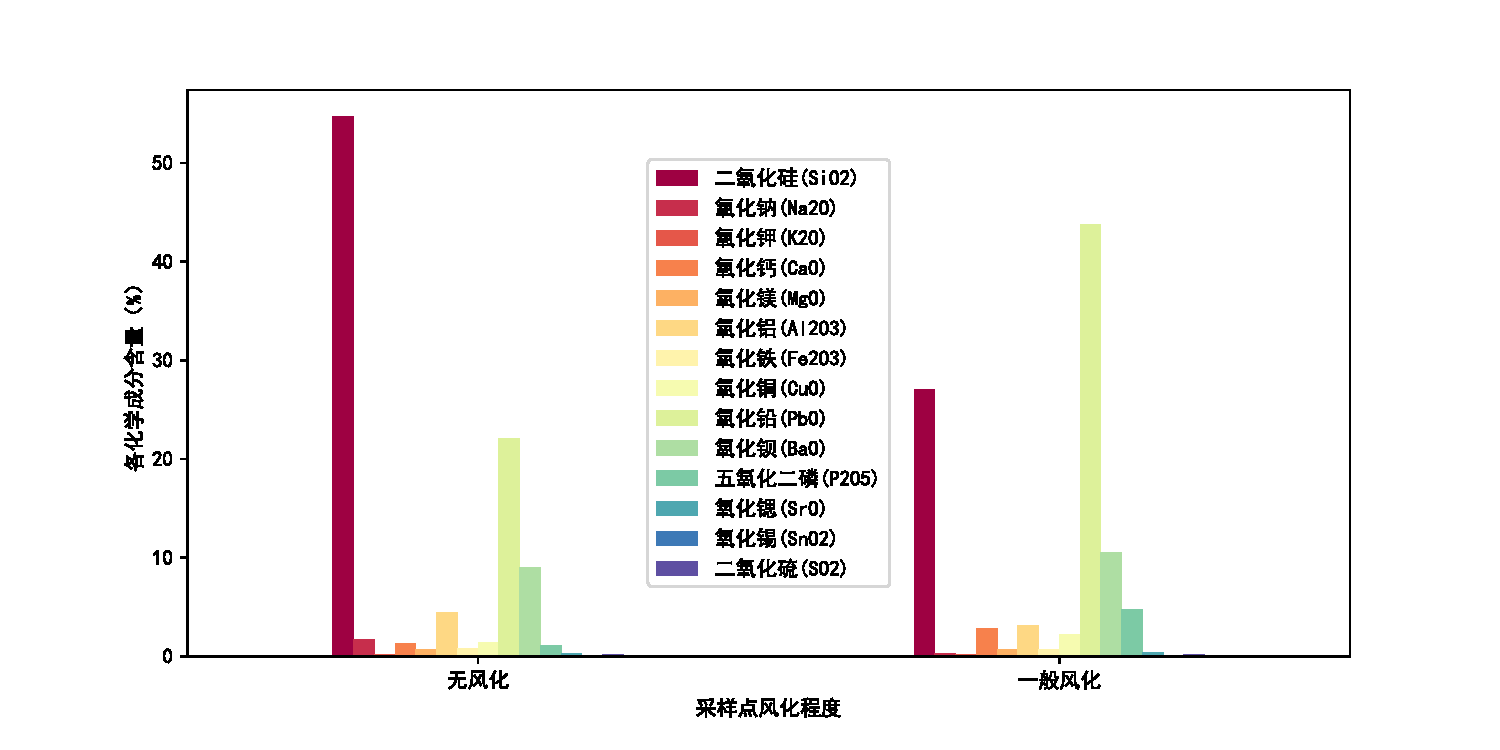
\includegraphics[scale=0.25]{铅钡玻璃含量平均值一般风化前后对比.pdf}
        \caption{铅钡玻璃含量平均值一般风化前后对比}
    \end{subfigure}
    \begin{subfigure}{0.4\textwidth}
        \centering
        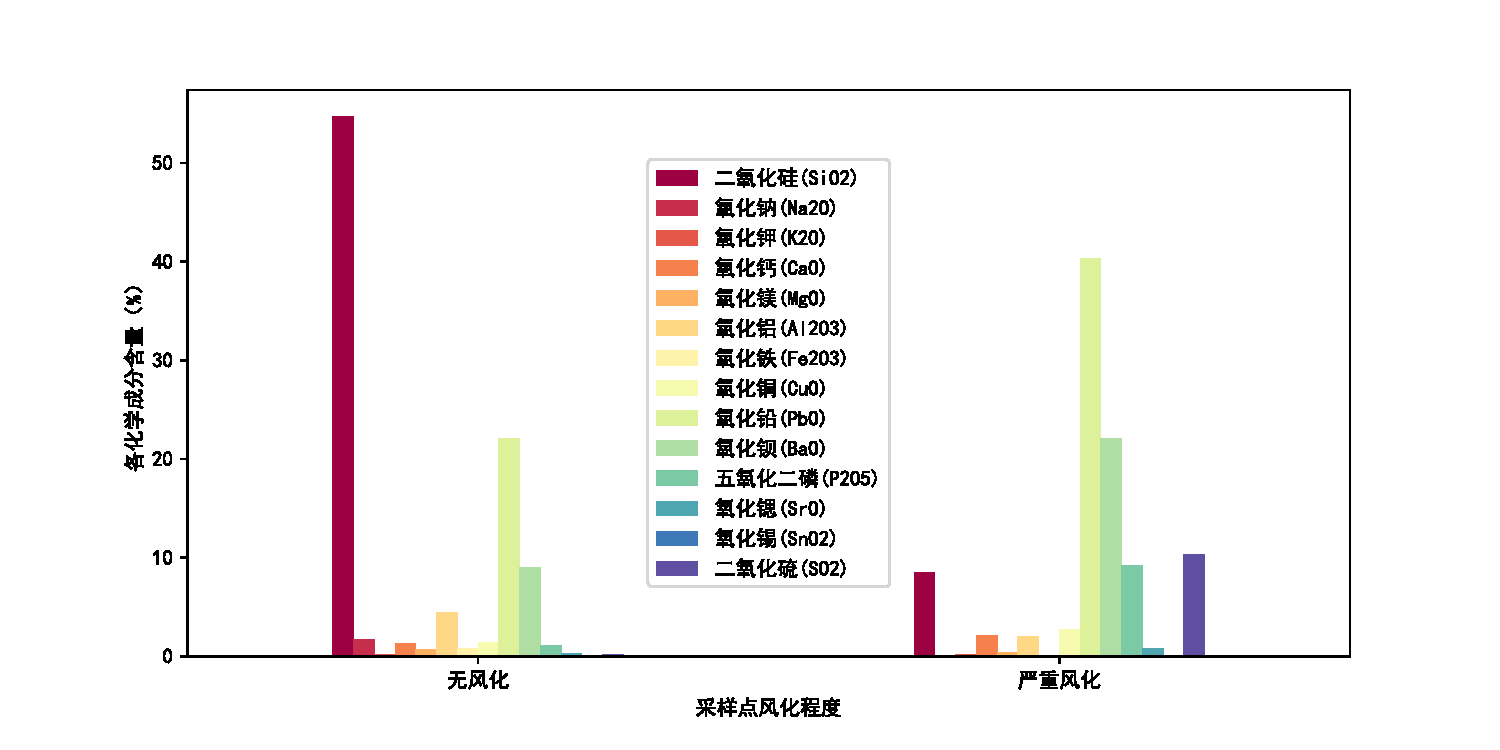
\includegraphics[scale=0.25]{铅钡玻璃含量平均值严重风化前后对比.pdf}
        \caption{铅钡玻璃含量平均值严重风化前后对比}
    \end{subfigure}
    \caption{风化前后各含量平均值变化规律}
    \label{fig:0}
\end{figure}
\begin{figure}[!htb]
    \centering
    \begin{subfigure}{0.4\textwidth}
        \centering
        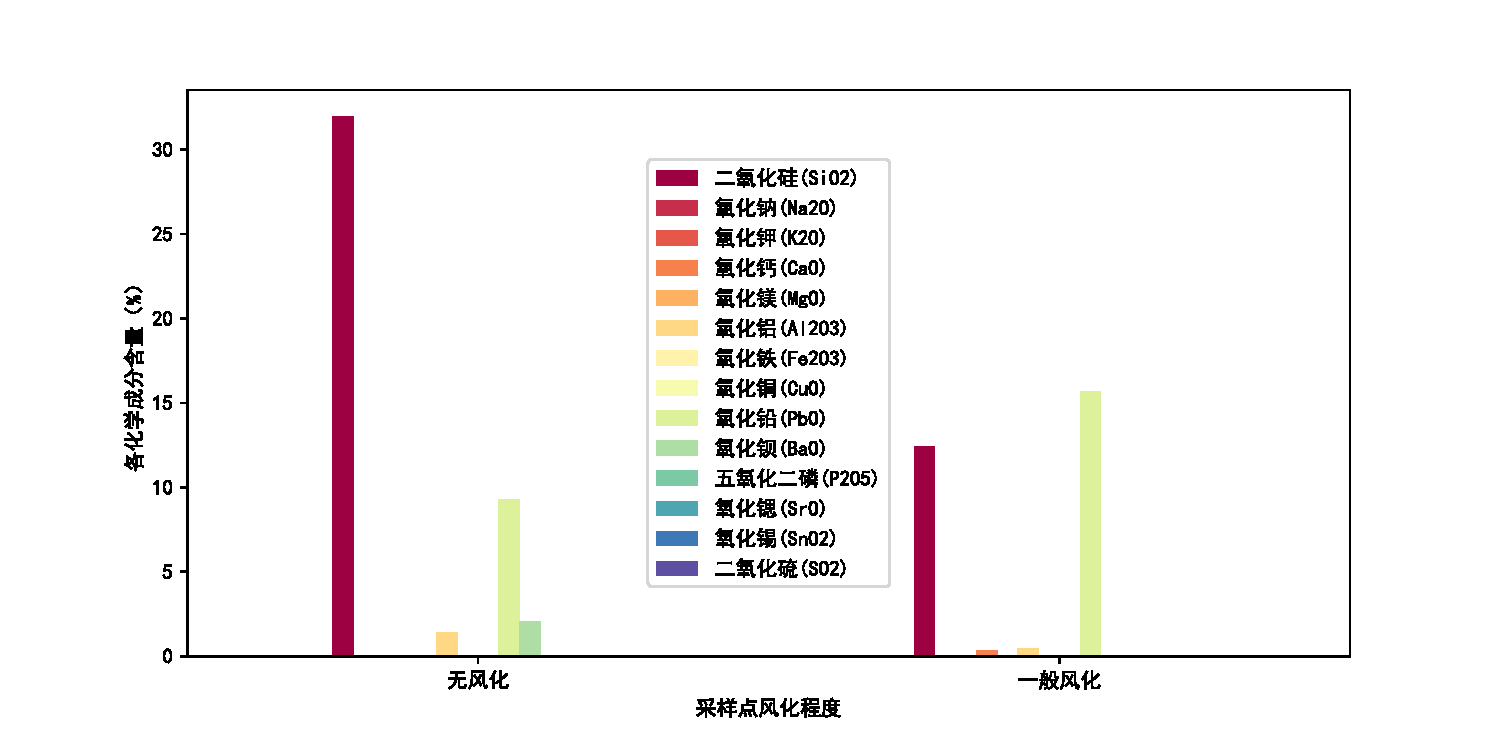
\includegraphics[scale=0.25]{铅钡玻璃含量最小值一般风化前后对比.pdf}
        \caption{铅钡玻璃含量最小值一般风化前后对比}
    \end{subfigure}
    \begin{subfigure}{0.4\textwidth}
        \centering
        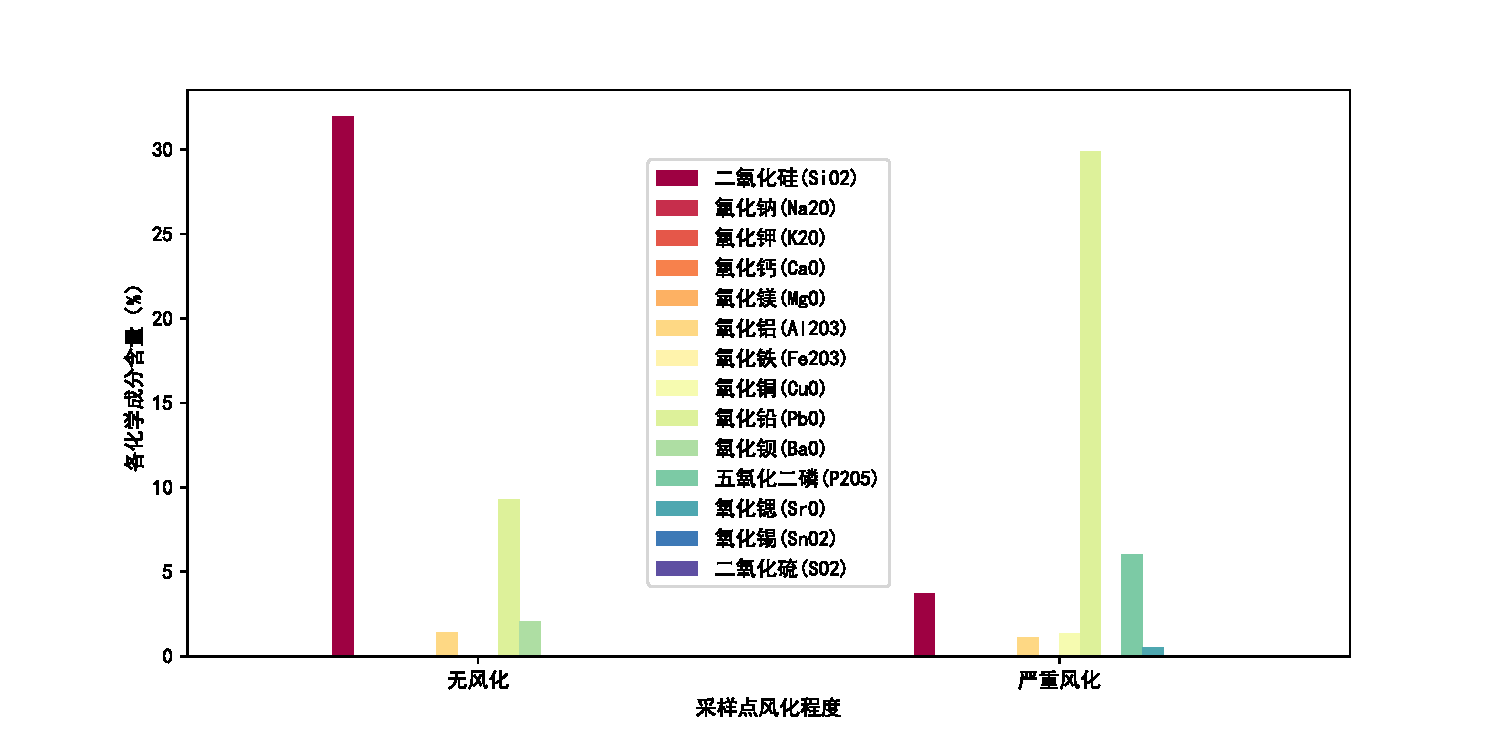
\includegraphics[scale=0.25]{铅钡玻璃含量最小值严重风化前后对比.pdf}
        \caption{铅钡玻璃含量最小值严重风化前后对比}
    \end{subfigure}
    \caption{风化前后各含量最小值变化规律}
    \label{fig:1}
\end{figure}
\begin{figure}[!htb]
    \centering
    \begin{subfigure}{0.4\textwidth}
        \centering
        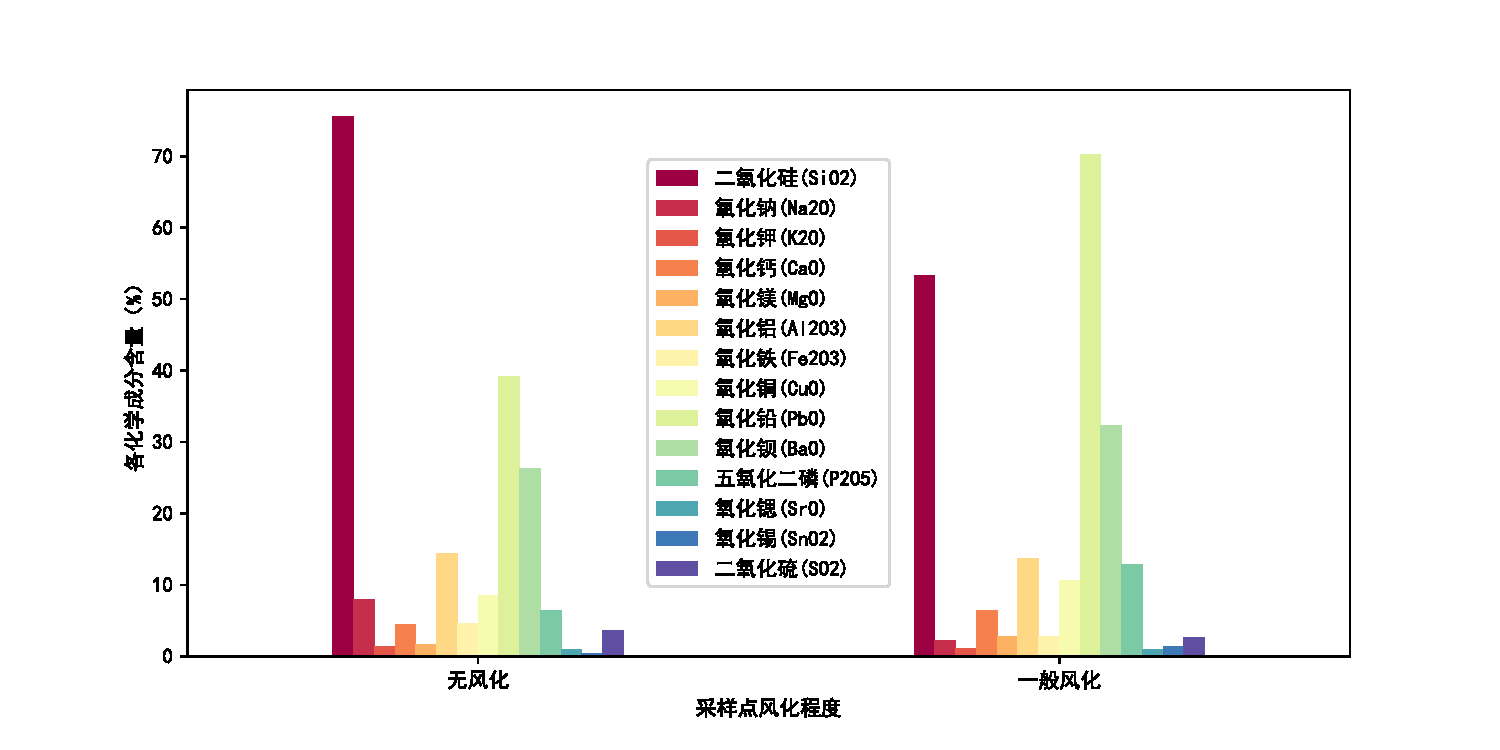
\includegraphics[scale=0.25]{铅钡玻璃含量最大值一般风化前后对比.pdf}
        \caption{铅钡玻璃含量最大值一般风化前后对比}
    \end{subfigure}
    \begin{subfigure}{0.4\textwidth}
        \centering
        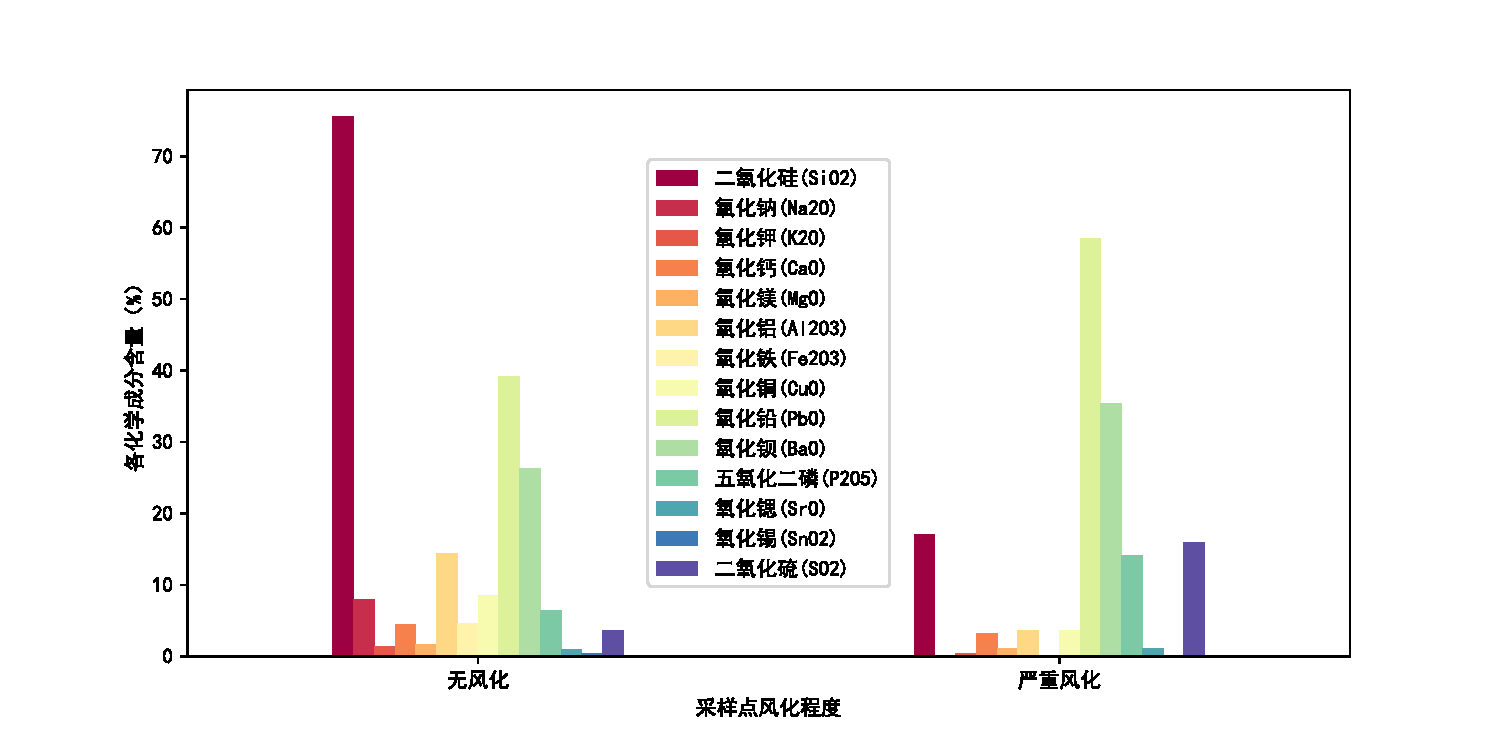
\includegraphics[scale=0.25]{铅钡玻璃含量最大值严重风化前后对比.pdf}
        \caption{铅钡玻璃含量最大值严重风化前后对比}
    \end{subfigure}
    \caption{风化前后各含量最大值变化规律}
    \label{fig:2}
\end{figure}

通过变化规律可以观测出,风化前后各含量最小值的有用性很低,由于多次出现风化
前后均为0的情况,许多成分的变化规律难以显示。风化前后各含量最大值在大小分
析上占有优势,但是结合实际数据发现,有多个成分的最大值为离群值,并不具有普
适性。相比最小值和最大值的变化规律,风化前后各含量平均值的变化既较好地匹配
了众多采样点的信息,又有足够用于统计规律的非零数据,因此选择风化前后各含量
平均值这组数据进行进一步的规律拟合。

\subsubsection{铅钡玻璃一般风化还原预测}
考虑到物质守恒和质量占比,在风化过程中,即使有少量的化学成分会脱落,但是大致
含量可以稳定。这里我们采取了两种一维拟合方式:加减法和乘除法,公式分别为:
\begin{equation}
    p_{m,s0}=p_{m,s1}-b_m \label{eq:0}
\end{equation}
\begin{equation}
    p_{m,s0}=p_{m,s1}\times k_m \label{eq:1}
\end{equation}

其中,$m$ 为采样点化学成分,$s$ 表示采样点风化状态,$s1$ 为一般风化后的状态,
$s0$ 为一般风化前的状态,这里我们用无风化的状态来等价一般风化前的状态。
$p_{m,s}$表示某化学成分$m$在采样点风化状态$s$下的含量。

根据风化前后各含量平均值,我们可以计算得到:
\begin{equation}
    b_m=\overline{p}_{m,s1}-\overline{p}_{m,s0},\qquad m=\mathrm{SiO_2,NaO_2,KO_2,\dots,SO_2}
    \label{eq:2}
\end{equation}
\begin{equation}
    k_m=\overline{p}_{m,s0}\div\overline{p}_{m,s1},\qquad m=\mathrm{SiO_2,NaO_2,KO_2,\dots,SO_2}
    \label{eq:3}
\end{equation}

考虑到实际情况中 $\overline{p}_{m,s1}$ 可能为 0,因此将式 \eqref{eq:3} 改为 
\[
    k_m=\overline{p}_{m,s0}\div(\overline{p}_{m,s1}+1\times 10^{-9})
\]

另外,在实际应用中由于 $\overline{p}_{m,s1}-b_m$ 可能会小于 0,不符合实际情况,因此式 
\ref{eq:0} 改为
\[
    p_{m,s0}=\max(0,p_{m,s1}-b_m)
\]

在实际数据中,对49号文物的一般风化部位的每个化学成分用公式 \eqref{eq:2},\eqref{eq:3}
分别拟合,得到各个化学成分风化前的含量,以49号文物无风化部位的各成分含量为标准,求取
所有化学成分含量预测总误差:
\begin{equation*}
    \mathrm{err}=\sqrt{\frac{\sum_{m=\mathrm{SiO_2}}^{\mathrm{SO_2}}
            (p_{m,s0}-p_{m,s1})^2}{14}}
\end{equation*}

\subsubsection{铅钡一般风化还原评估}
使用 49 号文物的无风化部位和一般风化部位进行验证,通过总误差计算公式和
得到:以公式 \eqref{eq:0} 拟合的误差为:11.323226600781831\%,公式 \eqref{eq:1} 的拟合
误差为:7.4257-12790211058\%。

同理,使用 50 号文物的无风化部位和一般风化部位进行验证,得到公式 \eqref{eq:0} 的拟合误
差为:13.136575761528826\%,公式 \eqref{eq:1} 的拟合误差为:23.30939253278124\%。

则公式 \eqref{eq:0} 的拟合误差平均值为 12.2299011811553285\%,公式 \eqref{eq:1} 的
拟合误差平均值为 15.367552661496149\%,公式 \eqref{eq:0} 的拟合误差方差为
0.8220587946954577\%,公式 \eqref{eq:1} 的拟合误差方差为 63.07282054113358\%。

由此可以得知公式 \eqref{eq:0} 的拟合效果更好,故用公式 \eqref{eq:0} 对其他一般风化采样
点进行预测风化前的各化学成分含量,得到结果\emph{铅钡玻璃一般风化复原.xlsx}。

\subsubsection{铅钡严重风化还原预测}
考虑到物质守恒和质量占比,在风化过程中,即使有少量的化学成分会脱落,但是大致含量
可以稳定。结合一般风化还原预测的效果,这里我们采取了加减法拟合方式:
\begin{equation}
    p_{m,s0}=p_{m,s2}-b_m
    \label{eq:4}
\end{equation}

其中,$m$ 为采样点化学成分,$s$ 表示采样点风化状态,$s1$ 为严重风化后的状态,$s0$ 为
一般风化前的状态,这里我们用无风化的状态来等价严重风化前的状态。$p_{m,s}$ 表示某化
学成分 $m$ 在采样点风化状态 $s$ 下的含量。

根据风化前后各含量平均值,我们可以计算得到:
\begin{equation*}
    b_m=\overline{p}_{m,s2}-\overline{p}_{m,s0},\qquad
    m=\mathrm{SiO_2,NaO_2,KO_2,\dots,SO_2}
\end{equation*}

由于实际情况下化学成分含量不为负数,因此应用公式 \eqref{eq:4} 时应变形为:
\[
    p_{m,s0}=\max(0,p_{m,s2}-b_m)
\]

用公式 \eqref{eq:4} 对其他一般风化采样点进行预测风化前的各化学成分含量,得到结
果\emph{铅钡玻璃严重风化复原.xlsx}。

\subsubsection{高钾玻璃风化规律观测}
从有效数据选出玻璃类型为高钾的采样点。然后将所有采样点根据风化程度分别划分为:无风化、
一般风化两种情况,这两组数据分别以无风化-一般风化、无风化-严重风化的方式进行匹配,
共得到两组用于拟合变换规律的数据。

同样,对这组验证数据进行和拟合用数据相同的处理,把缺失信息填充为 0。

在拟合变换规律之前,我们首先求取了用于拟合变换规律的三组数据的各种成分在不同采样点
的最小值、平均值、最大值,从而绘制了无风化与一般风化的采样点化学成分含量图,作为
寻找规律的前提,如图 \ref{fig:HighKaverage}、\ref{fig:HighKmin}、\ref{fig:HighKmax}
所示。
\begin{figure}[!htb]
    \centering
    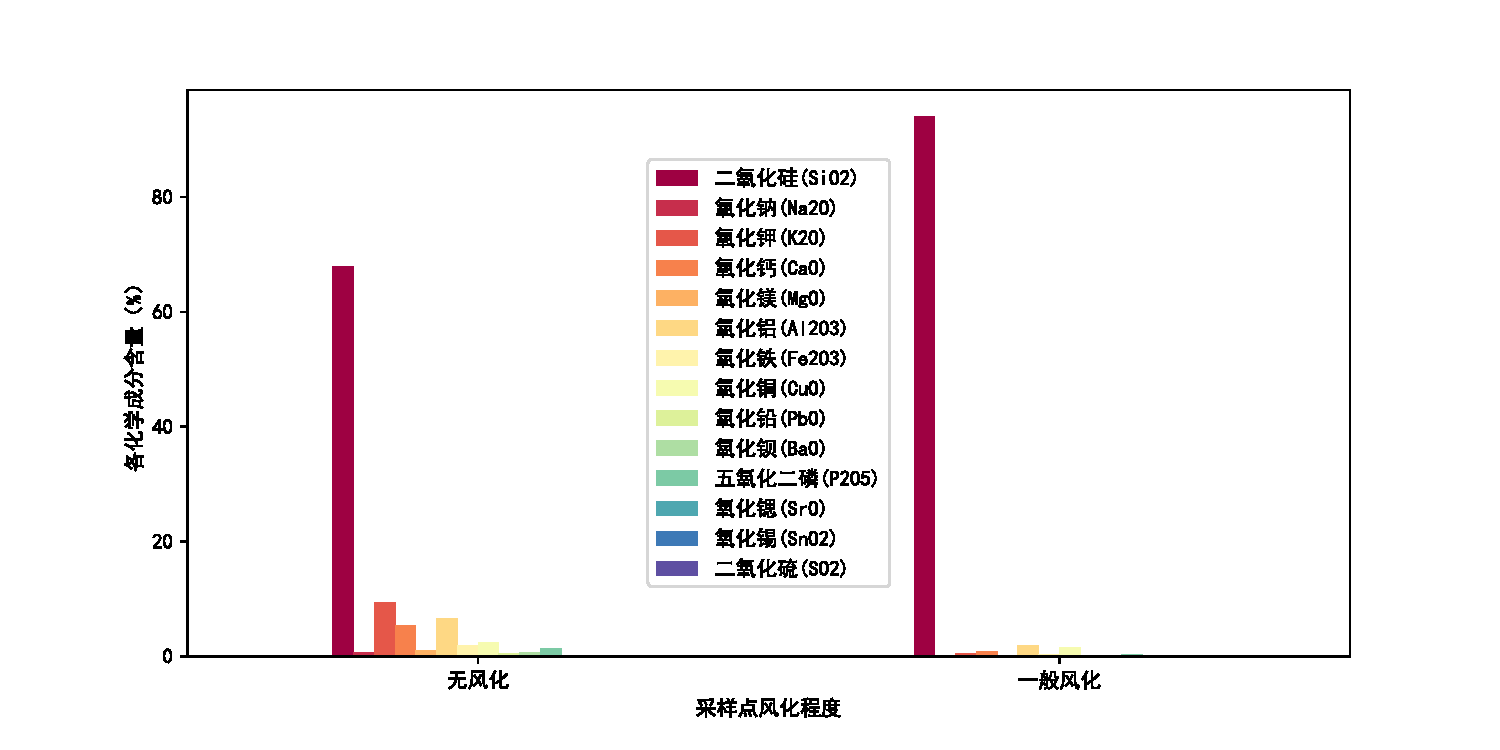
\includegraphics[scale=0.35]{高钾玻璃含量平均值一般风化前后对比.pdf}
    \caption{风化前后各含量平均值变化规律}
    \label{fig:HighKaverage}
\end{figure}
\begin{figure}
    [!htb]
    \centering
    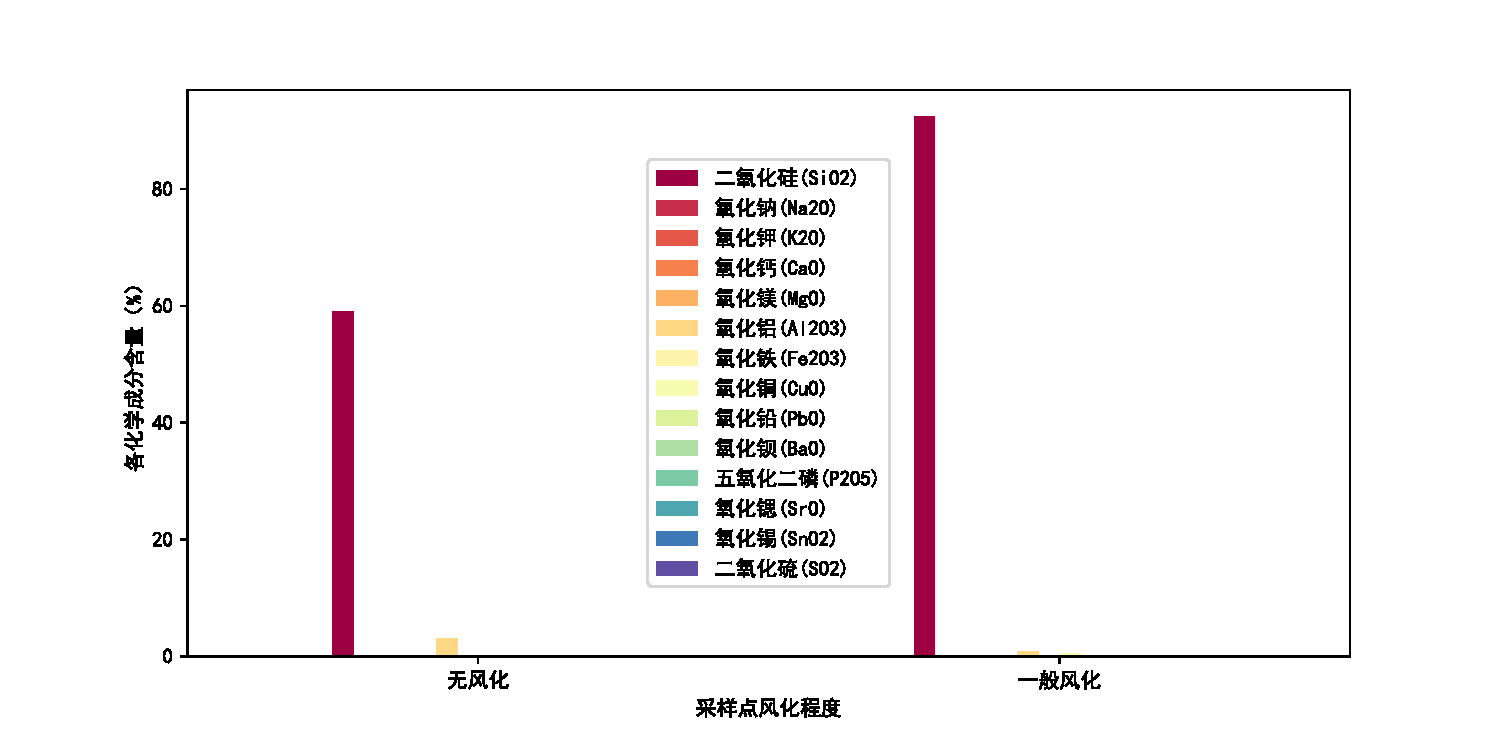
\includegraphics[scale=0.35]{高钾玻璃含量最小值一般风化前后对比.pdf}
    \caption{风化前后各含量最小值变化规律}
    \label{fig:HighKmin}
\end{figure}
\begin{figure}
    [!htb]
    \centering
    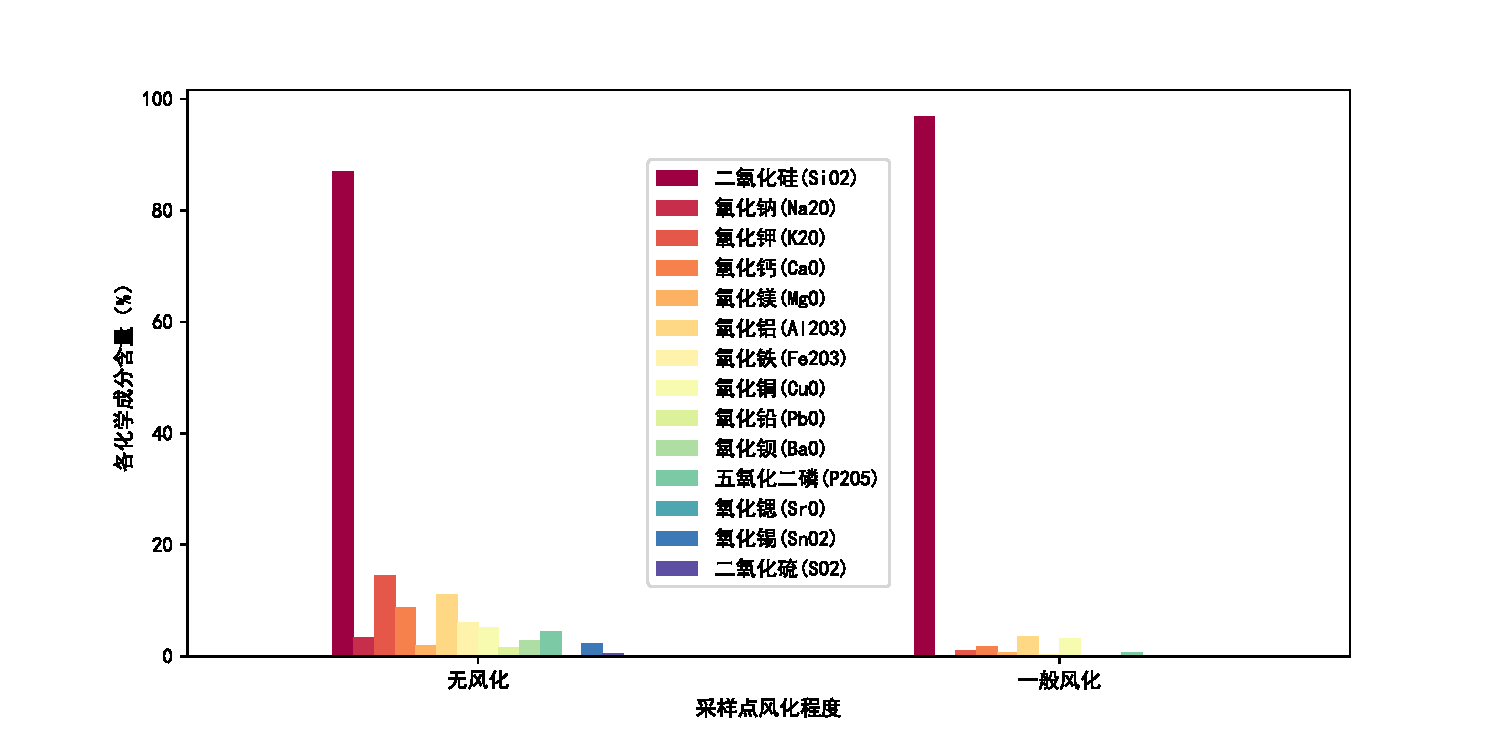
\includegraphics[scale=0.35]{高钾玻璃含量最大值一般风化前后对比.pdf}
    \caption{风化前后各含量最大值变化规律}
    \label{fig:HighKmax}
\end{figure}

通过变化规律可以观测出,高钾玻璃风化前后各含量的变化与铅钡玻璃有一定
的相似性,相比最小值和最大值的变化规律,风化前后各含量平均值的变化既
较好地匹配了众多采样点的信息,又有足够用于统计规律的非零数据,因此选
择风化前后各含量平均值这组数据进行进一步的规律拟合。

\subsubsection{高钾玻璃一般风化还原预测}
考虑到物质守恒和质量占比,在风化过程中,即使有少量的化学成分会脱落,
但是大致含量可以稳定。结合铅钡玻璃中的效果,这里我们采取了一维拟合方
式:加减法,公式为:
\begin{equation}
    p_{m,s0}=p_{m,s1}-b_m
    \label{eq:a0}
\end{equation}

其中,$m$ 为采样点化学成分,$s$ 表示采样点风化状态,$s1$ 为一般风化后的
状态,$s0$ 为一般风化前的状态,这里我们用无风化的状态来等价一般风化前的
状态。$p_{m,s}$ 表示某化学成分 $m$ 在采样点风化状态 $s$ 下的含量。

根据风化前后各含量平均值,我们可以计算得到:
\begin{equation}
    b_m = \overline{p}_{m,s1}-\overline{p}_{m,s0},\qquad 
    m=\mathrm{SiO_2,NaO_2,KO_2,\dots,SO_2}
    \label{eq:a1}
\end{equation}

由于实际情况下化学成分含量不为负数,因此应用公式 \eqref{eq:a0} 时变形为:
\[
    p_{m,s0}=\max(0,p_{m,s1}-b_m)
\]

用公式 \eqref{eq:a0} 对其他一般风化采样点进行预测风化前的各化学成分含
量,得到结果\emph{高钾玻璃一般风化复原.xlsx}。


\subsection{高钾玻璃、铅钡玻璃的分类规律}
\subsubsection{模型建立}
根据图 \ref{fig:all0} 可知:风化因子对不同化学成分含量的影
响远小于玻璃类型的影响,因此不需要对风化和无风化的采样点分别处理。
\begin{figure}[!htb]
    \centering
    \begin{subfigure}{0.45\textwidth}
        \centering
        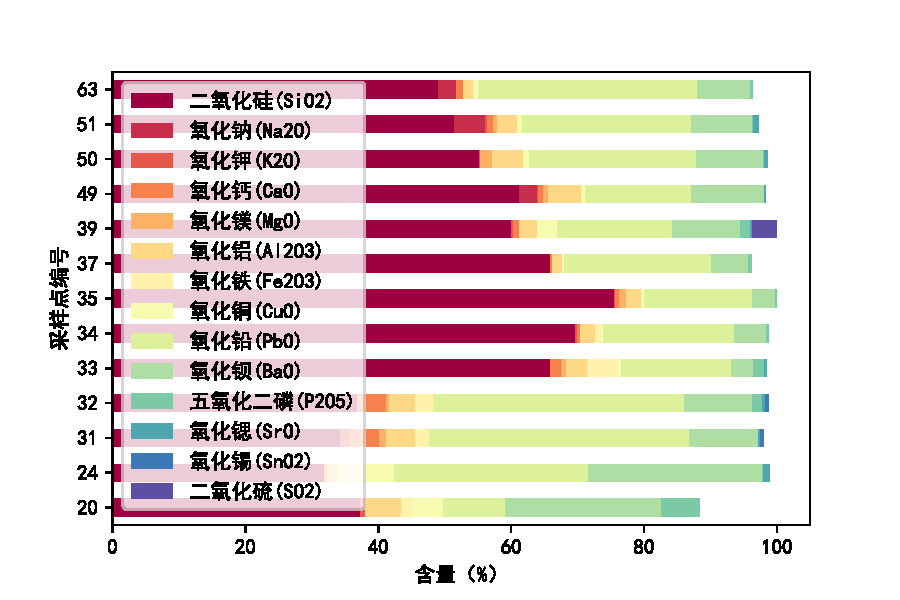
\includegraphics[scale=0.45]{铅钡无风化.pdf}
        \caption{铅钡玻璃风化前含量图}
    \end{subfigure}
    \qquad
    \begin{subfigure}{0.45\textwidth}
        \centering
        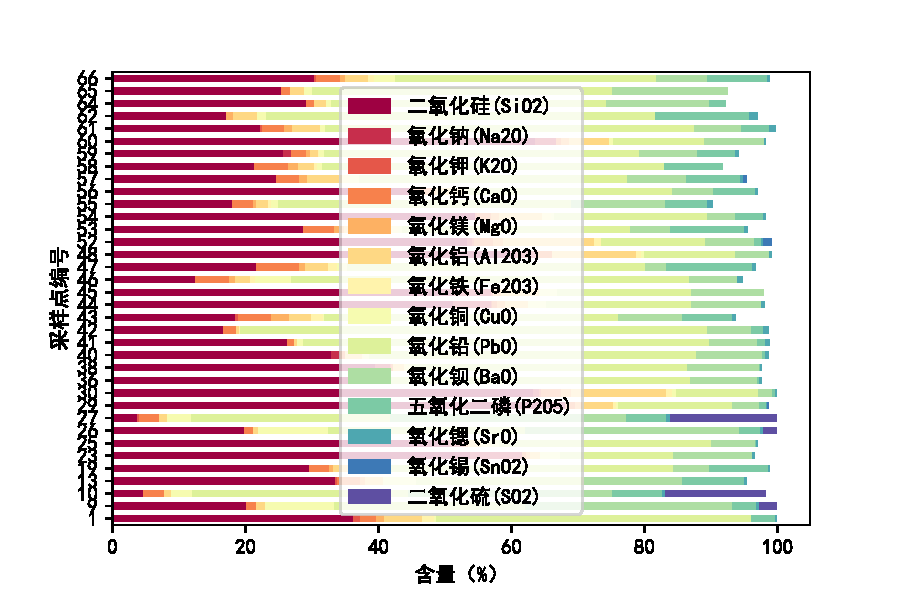
\includegraphics[scale=0.45]{铅钡风化.pdf}
        \caption{铅钡玻璃风化后含量图}
    \end{subfigure} \\[10pt]
    \begin{subfigure}{0.45\textwidth}
        \centering
        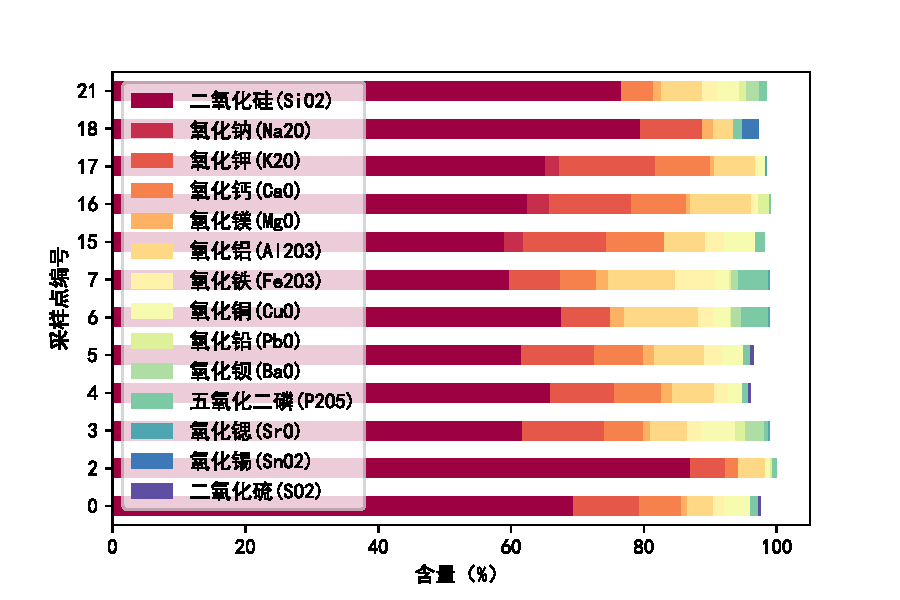
\includegraphics[scale=0.45]{高钾无风化.pdf}
        \caption{高钾玻璃风化前含量图}
    \end{subfigure}
    \qquad
    \begin{subfigure}{0.45\textwidth}
        \centering
        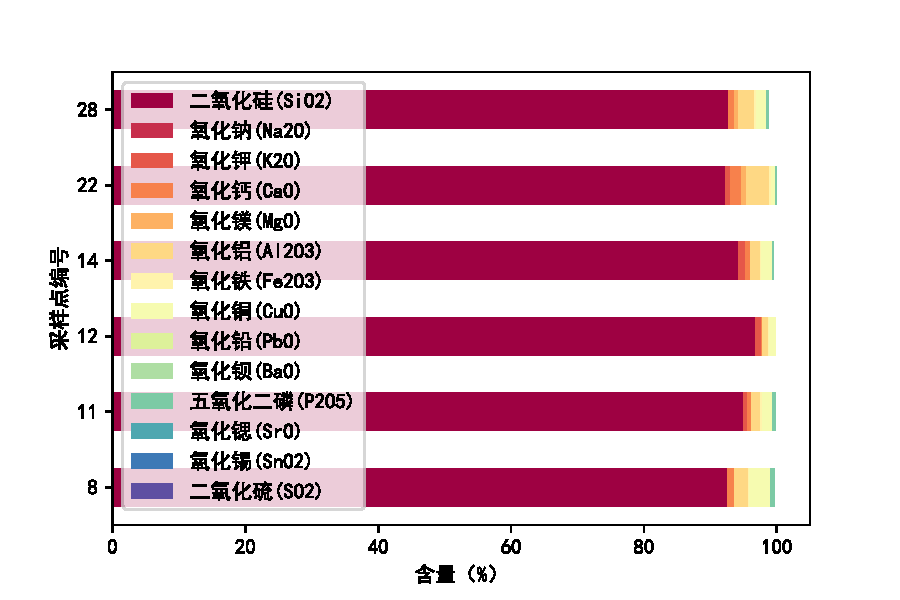
\includegraphics[scale=0.45]{高钾风化.pdf}
        \caption{高钾玻璃风化后含量图}
    \end{subfigure}
    \caption{不同类型玻璃风化前后的各化学成分含量}
    \label{fig:all0}
\end{figure}

首先,我们将离散文本变量作数值化处理,将玻璃类型中的“高钾”对应数字0,
“铅钡”对应数字1。

我们的优化目标是:将根据化学成分含量预测出高钾玻璃和铅钡玻璃的划分误差
最小,将划分误差统计函数用 $L$ 表示,则有公式:
\[
    \min_{f\in F}\frac{1}{N}\sum_{i=1}^NL(y_i,f(x_i))
\]

这里我们使用交叉熵作为分类问题的损失函数:
\[
    L=\sum_{i=1}^Ny^{(i)}\log\widehat{y}^{(i)}+(1-y^{(i)})\log(1-\widehat{y}^{(i)})
\]

将 CART 回归树作为基分类器,对于每个 CART 树,有:
\[
    obj(t)=-\frac{1}{2}\sum_{j=1}^T\frac{G_j^2}{H_j+\lambda}+\gamma T
\]

其中,$G_j$ 表示映射为叶子节点 $j$ 的所有输入样本的预测误差对当前模型的一阶
导之和,同理,$H_j$ 表示二阶导之和,$\gamma$ 表示节点切分的难度,$\lambda$
表示 $L_2$ 正则化系数,$T$ 为叶子节点的个数。

对于每个叶节点,通过增加该节点后交叉熵的损失程度,表示划分所得到的增益,对应
公式为:
\begin{align*}
    \mathrm{Gain} & =Obj_{L+R}-(Obj_L+Obj_R)                                                 \\
                  & =\left[-\frac{1}{2}\frac{(G_L+G_R)^2}{H_L+H_R+\lambda}+\gamma T\right] -
    \left[\frac{1}{2}(\frac{G_L^2}{H_L+\lambda}+\frac{G_R^2}{H_R+\lambda})+
    \gamma(T+1)\right]                                                                       \\
                  & =\frac{1}{2}\left[\frac{G_L^2}{H_L+\lambda}+\frac{G_R^2}{H_R+\lambda}-
        \frac{(G_L+G_R)^2}{H_R+H_L+\lambda}\right]-\gamma
\end{align*}

对于不同CART树,$f^t(x_i)$ 为第 $t$ 棵树的输出结果,$\widehat{y}_i^{(t)}$是
模型当前的输出结果,$y_i$ 是实际的结果,有:
\begin{gather*}
    \widehat{y}_i^{(t)}=\sum_{t=1}^tf^t(x_i) \\
    \widehat{y}_i^{(t)}=\widehat{y}_i^{(t-1)}+f^t(x_i)
\end{gather*}

对于所有CART树,通过最小化损失函数来构建最优模型,加入复杂度惩罚项防止过拟
合,则有:
\[
    obj(t)=\sum_{i=1}^nL(y_i,\widehat{y}_i)+\Omega(f(t))+Constant
\]

特征在作为划分属性时 Loss 平均的降低量(也就是特征的信息增益),以特征
$k=1,2,...,K$ 为例,其重要度计算可以表述如下:
\begin{equation}
    V(k)=\frac{1}{2}\frac{\displaystyle \sum_{t=1}^T\sum_{i=1}^N(t)
    I(\beta(t,i)=k)(\frac{G^2_{\gamma(t,i,L)}}{H_{\gamma(t,i,L)+\lambda}}+
    \frac{G^2_{\gamma(t,i,R)}}{H_{\gamma(t,i,R)+\lambda}}-
    \frac{G^2_{\gamma(t,i)}}{H_{\gamma(t,i)+\lambda}})}
    {\displaystyle \sum_{t=1}^T\sum_{i=1}^{N(t)}I(\beta(t,i)=k)}
    \label{eq:importanceCalculate}
\end{equation}
\indent 这里k表示某节点,$T$ 表示所有树的数量,$N(t)$ 表示第 $t$ 棵树的非叶子节点数量,
$\beta(t,i)\in 1,2,\dots,K$ 表示第 $t$ 棵树的第 $i$ 个非叶子节点的划分特征,
$I(\beta(t,i)=k)$ 是指示函数,分别表示落在第 $t$ 棵树的第 $i$ 个非叶子节点上所有样
本的一阶导数和二阶导数之和,分别表示落在第 $t$ 棵树上第 $i$ 个非叶子节点的左、右节点
上的一阶导数之和,同理,分别表示落在第 $t$ 棵树上第 $i$ 个非叶子节点的左、右节点上的
二阶导数之和,所以有
\[
    G_{\gamma(t,i)}=G_{\gamma(t,i,L)}+G_{\gamma(t,i,R)},
    H_{\gamma(t,i)}=H_{\gamma(t,i,L)}+H_{\gamma(t,i,R)}
\]
\indent $\lambda$ 为正则化项的超参数。

\subsubsection{模型求解}
通过遍历和梯度更新,对于每个 CART 回归树,采用贪心算法,每次选取分割后可以获取最大
增益的叶节点进行分割,从而将每个样本映射到唯一确定的一个叶子节点中,同一叶子节点中
的所有样本共享相同的预测值。

XGBoost 不断生成新的 CART 回归树,每生成一颗树则学习一个新的函数,函数的目标则是
去拟合所有叶子节点中样本的历史残差。

采用 80\% 的数据作为训练数据,20\% 的数据作为测试数据,所得模型在训练集和测试集
中表现分别如表 \ref{tab:train}、表 \ref{tab:test}。
\begin{table}[!htb]
    \centering
    \begin{tabular}{|c|c|c|c|c|c|}
        \hline
        Accuracy & Precision & Recall   & F        & AUC      & KS       \\
        \hline
        100.00\% & 100.00\%  & 100.00\% & 100.00\% & 100.00\% & 100.00\% \\
        \hline
    \end{tabular}
    \caption{训练集效果}
    \label{tab:train}
\end{table}
\begin{table}[!htb]
    \centering
    \begin{tabular}{|c|c|c|c|c|c|}
        \hline
        Accuracy & Precision & Recall   & F        & AUC      & KS       \\
        \hline
        100.00\% & 100.00\%  & 100.00\% & 100.00\% & 100.00\% & 100.00\% \\
        \hline
    \end{tabular}
    \caption{测试集效果}
    \label{tab:test}
\end{table}

模型的所有指标评估在训练集和测试集上效果均为 100\%,可知模型获得了极好的效果,可以
应用于获取特征重要性。通过重要度计算公式 \eqref{eq:importanceCalculate} 可以得到
不同化学成分在划分玻璃类型的规律。

\subsubsection{模型分析}
将所得不同化学成分在划分玻璃类型的规律可视化,如图 \ref{fig:visual0}
\begin{figure}[!htb]
    \centering
    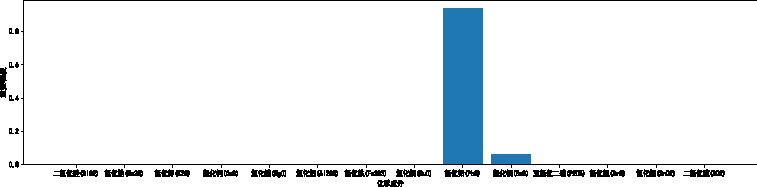
\includegraphics{不同化学成分在划分玻璃类型的规律.pdf}
    \caption{不同化学成分在划分玻璃类型的规律}
    \label{fig:visual0}
\end{figure}

从图 \ref{fig:visual0} 中可知,氯化铅和氯化钡在划分不同玻璃类型的过程中起到
了重要作用,尤其是
$\mathrm{PbO}$ ,其含量与铅钡类型具有强烈的正相关性质。结合最初可视化的图,
同时考虑到“铅钡”类型的玻璃与 PbO 和 BaO 中的元素直接相关,可知,结论合理。
同时考虑到最初可视化的图片中 $\mathrm{SiO_2}$ 的含量在不同类型中的明显变
化,我们将 PbO 和 BaO 两个特征去除后再次进行了模型训练,发现各项指标在训练
集仍然为100\%,但在测试集表 \ref{tab:test1} 中有所下降。
\begin{table}[!htb]
    \centering
    \begin{tabular}{|c|c|c|c|c|c|}
        \hline
        Accuracy & Precision & Recall  & F       & AUC     & KS      \\
        \hline
        94.12\%  & 100.00\%  & 92.31\% & 96.00\% & 96.15\% & 92.31\% \\
        \hline
    \end{tabular}
    \caption{PbO 和 BaO 两个特征去除后的测试集效果}
    \label{tab:test1}
\end{table}

这表明我们对于特征重要程度的划分存在合理性,失去这两项重要特征后模型分类效果的
确下降,同时也证明了其他化学成分含量特征与玻璃类型分类也存在一定的关联规律,再
次通过重要度计算公式可以得知剩余成分在划分玻璃类型的规律,可视化如图
\ref{fig:visual1}。
\begin{figure}[!htb]
    \centering
    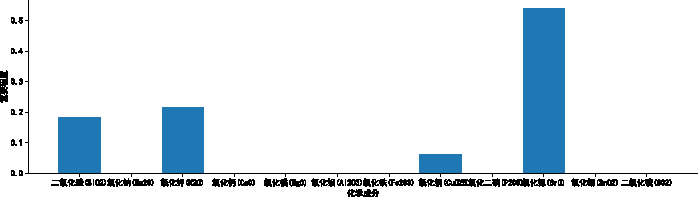
\includegraphics{剩余成分在划分玻璃类型的规律.pdf}
    \caption{剩余成分在划分玻璃类型的规律}
    \label{fig:visual1}
\end{figure}

通过图示可知,SrO 在划分玻璃类型中也起到了重要作用,$\mathrm{SiO_2}$ 和 
$\mathrm{K_2O}$ 作用相
对其较小,CuO 也与玻璃类型有一定的关联规律。结合图 \ref{fig:averageContent}
可知,在高钾玻璃中 SrO 含量比较明显,而在铅钡玻璃中 SrO 接近于无,同时
 $\mathrm{SiO_2}$、$\mathrm{K_2O}$ 
和 CuO 在高钾玻璃中的含量也明显高于在铅钡玻璃中的含量。进一步证明了
规律的合理性。
\begin{figure}[!htb]
    \centering
    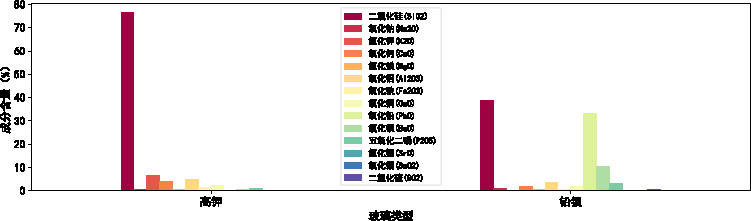
\includegraphics{高钾和铅钡玻璃中各成分平均含量示意图.pdf}
    \caption{高钾和铅钡玻璃中各成分平均含量示意图}
    \label{fig:averageContent}
\end{figure}

因此,我们总结规律如下,设划分至当前类为取值 1,含量增加为正增长,则 PbO 和 BaO 的含量
与划分为铅钡玻璃具有明显的正相关性;比之较弱的还有 SrO,与高钾玻璃划分具有明显
的正相关;其次是 $\mathrm{Si_2O}$ 和 $\mathrm{K_2O}$ ,受风化程度对二者在铅钡玻璃中提升带来波
动的影响,其与高钾玻璃划分具有正相关性,但是较弱,如果区分不同风化程度下玻璃类型
的划分,可能规律性会更强一些,但是这种先划分风化程度后根据成分含量划分玻璃类型
的方式并不符合文物划分规律,因此并不进行进一步讨论;此外,CuO 也与高钾玻璃具有
一定的正相关性,但其同时在铅钡玻璃中也有明显存在,规律并不十分明显。

\subsection{高钾玻璃、铅钡玻璃的分类模型}
\subsubsection{数据预处理}
通过题目可知:在不同的文物中检测出的化学成分具有较大差别,附件表单 2 中的某些
成分可能只存在于部分文物样品上;附件表单 2 中数据具有成分性,由于检测手段和其他
因素可能导致比例累加和不严格等于 100\%,因此将成分比例累加和介于 85\%\~{}105\%
之间的数据视为有效数据。由此对数据进行以下预处理:
\begin{enumerate}
    \item 为提高数据的可使用性,对于缺失值使用固定值 0 进行填充,在保证其可
          以正常运算的同时不会影响数据真实性。
    \item 分析表单 2 中数据,对所有采样点的成分比例进行累加,发现编号 15 与
          17 的采样点的累加和不在 85\%\~{}105\% 之间,因此被视作无效数据并移除。
\end{enumerate}

\subsubsection{结合具体数据和聚类原理的过程分析}
对于每个类别选择合适的化学成分对其进行亚类划分采用的 K-means 聚类算法。

接下来对算法进行分析。

首先选择初始化的 $k$ 个样本作为初始的聚类中心,聚类中心为随机生成。
\[
    M^{(0)}=\{m_1^{(0)},m_2{(0)},m_3^{(0)},\dots,m_n^{(0)}\}
\]

此处选择欧氏距离作为度量方法,计算方法如下:
\[
    d_{ij}=\sum_{k=1}^m(x_{ki}-x_{kj})^2
\]

我们定义样本与其聚类中心的距离和为损失函数,当聚类后达到损失函数要求后训
练将停止。

在第一次聚类中,计算每一个点与每一个聚类中心之间的欧氏距离,得出结果后,
对于每一个点划归与其最近的一个聚类。

对于第一次聚类结果,分别计算每一个类的均值以此成为新的聚类中心。
\[
    M^{\mathrm{epoch}}=\{m_1^{\mathrm{epoch}},m_2^{\mathrm{epoch}},
    m_3^{\mathrm{epoch}},m_4^{\mathrm{epoch}},\dots,m_n^{\mathrm{epoch}}\}
\]

重复上述聚类操作,直到满足损失函数或聚类模型已经收敛后停止训练。



\subsubsection{聚类的评估及选择}
虽然聚类并没有直接的评估方法。但是我们可以计算出聚类后簇之间的离散情况以及每
一簇内的聚集程度来评估聚类的效果。在此,我们采用两个指标 CH 和 轮廓系数。
CH 指标的定义为:
\[
    \mathrm{CH} = \frac{\text{数据集的分离度}}{\text{类内的紧密度}}
\]
\indent 类内的紧密度通过计算簇中各点与簇中心的距离平方和来度量,数据集的分离
度通过计算各簇中心点与数据集中心点距离平方和来度量。

对以上公式进行简要分析。当分离度不变时,紧密度提高,会使得分子不变,分母减小,
因此 CH 变大;当紧密度不变时,分离度提高,会使得分子变大,分母不变,因此 CH
变大。所以可得结论:CH 越大就意味着簇与簇之间分散程度大,簇之内更紧密,所以
聚类的效果也就更好。

轮廓系数同样也与内聚度和分离度两种因素有关。对于簇中的每个向量,可以计算出它的
轮廓系数。对于一个点 $i$,向量 $i$ 的轮廓系数为:
\[
    S(i)=\frac{b(i)-a(i)}{\max\{a(i),b(i)\}}
\]
\indent 其中,$a(i)$ 为平均簇内距离,即 average($i$ 向量到所有它属于的簇中
其它点的距离)。$a(i)$ 越小,说明样本 $i$ 越应该被聚类到该簇。$a(i)$ 被称为
样本 $i$ 的簇内不相似度。$b(i)$ 为样本点到与其最近的非此簇的距离。$b(i)$ 
越大,说明样本 $i$ 越不属于其他簇。很明显轮廓系数的值
属于[-1,1],越趋近于1,内聚度以及分离度就越好。对所有点的轮廓系数求平均,就
能够得到聚类结果总的轮廓系数。

观察图 \ref{fig:clusterEvaluation},可以得出分类数为 2 时效果最好,为 8 时
次之。因为题目默认的分类数为 2,所以我们选择分类数为 8。
\begin{figure}[!htb]
    \centering
    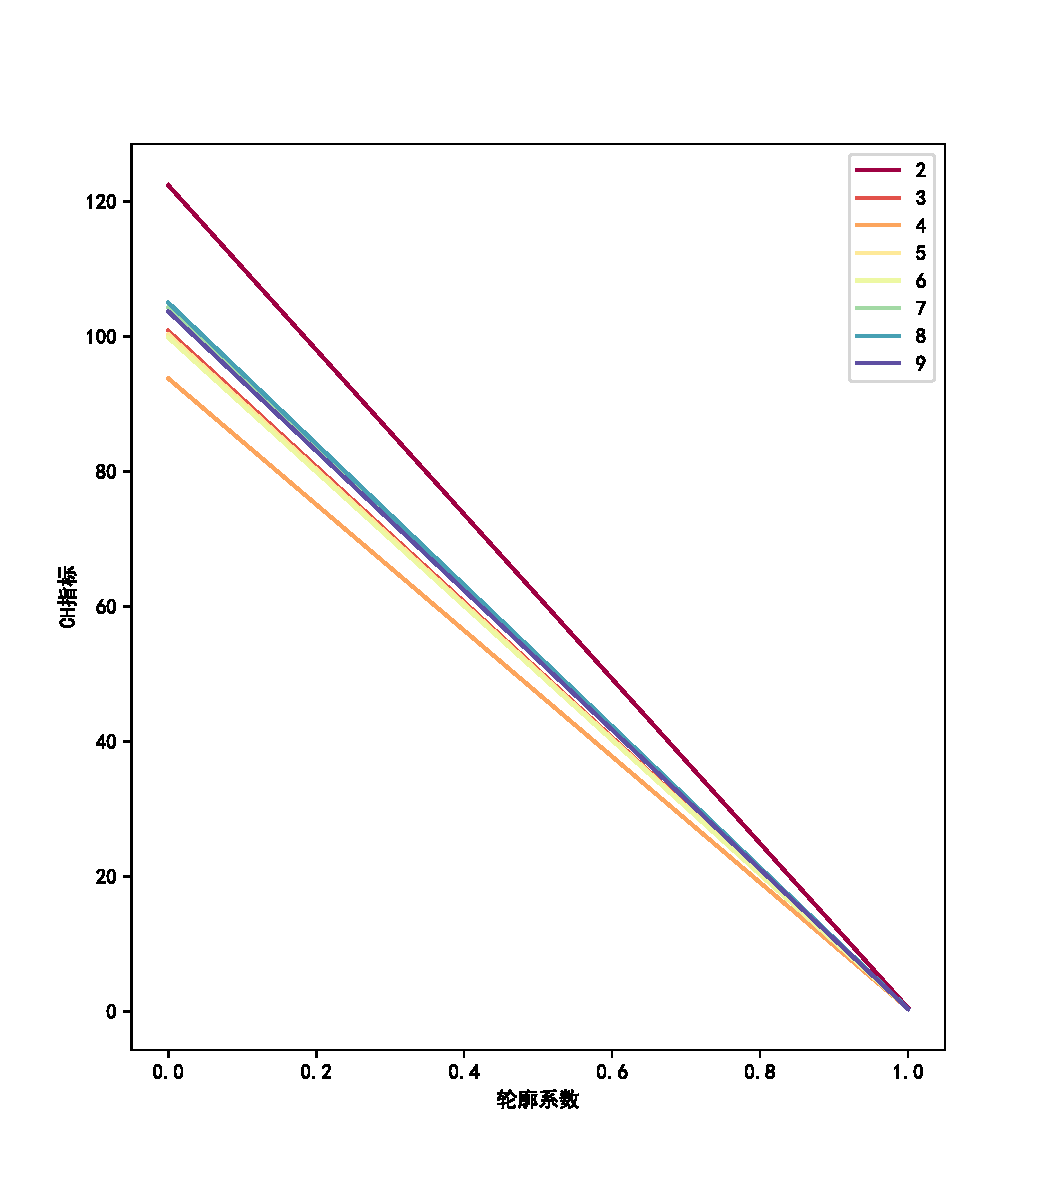
\includegraphics[scale=0.4]{聚类评估.pdf}
    \caption{聚类评估}
    \label{fig:clusterEvaluation}
\end{figure}

\subsubsection{聚类结果的分析}
将分类数为 8 的聚类进行 SPSS 分析,获得的结果见支持材料\emph{字段差异性分析.xlsx}。
观察表\emph{字段差异性分析.xlsx}中数据,我们可以用每一种化学成分对应每个分类类别的值来
度量该化学成分在该类别中所占的权重大小。平均值越大,意味着占据的权重越大,反之亦然。
根据此,可以得到类别 1 的玻璃主要化学成分为 $\mathrm{SiO_2(51.571\pm 3.001)}$,$
\mathrm{PbO(24.379\pm 6.021)}$,$\mathrm{BaO(8.482\pm 2.42)}$,类别 2 的玻璃
主要化学成分为 
$\mathrm{SiO_2}(89.663\pm 7.119)$,类别 3 的玻璃主要化学成分为 $\mathrm{SiO_2
(19.352\pm 4.906),PbO(59.392\pm 6.342)}$,类别 4 的玻璃主要化学成分为 
$\mathrm{SiO_2(60.295\pm 1.817),SnO_2(74.605\pm 30.172)}$,类别 5 的玻璃主
要化学成分为:$\mathrm{SiO_2}(29.488\pm 6.449)$,$\mathrm{PbO}(41.793±5.768)$,
类别 6 的玻璃主要化学成分为:$\mathrm{SiO_2}(65.422\pm 4.743)$,
$\mathrm{PbO}(16.447\pm 2.919)$,类别 7 的玻璃主要成分为:$\mathrm{SiO_2}
(64.576\pm 3.403)$,$\mathrm{K_2O}(10.554\pm 2.63)$,类别 8 的玻璃主要成分为:
$\mathrm{BaO}(29.888\pm 4.299)$,$\mathrm{PbO}(26.503±8.53)$,
$\mathrm{SiO_2}(19.593\pm 13.747)$。

根据分析不同类别中的化学含量差异,结合文献\cite{ref1,ref2},得出以下分类:
\begin{description}
    \item[类别 1] $\mathrm{PbO}$-$\mathrm{BaO}$-$\mathrm{SiO_2}$ 玻璃系统 1
    \item[类别 2] $\mathrm{K_2O}\mbox{-}\mathrm{SiO_2}$ 玻璃系统 4
    \item[类别 3] $\mathrm{PbO}\mbox{-}\mathrm{SiO_2}$ 玻璃系统 6
    \item[类别 4] $\mathrm{K_2O}$-$\mathrm{Na_2O}$-$\mathrm{CaO}$-$\mathrm{SiO_2}$ 玻璃系统 5
    \item[类别 5] $\mathrm{PbO\mbox{-}K_2O\mbox{-}BaO\mbox{-}P_2O_5\mbox{-}SiO_2}$ 玻璃系统 
    \item[类别 6] $\mathrm{Na_2O\mbox{-}CaO\mbox{-}PbO\mbox{-}SiO_2}$ 玻璃系统 7 
    \item[类别 7] $\mathrm{K_2O\mbox{-}Al_2O_3\mbox{-}Fe_2O_3\mbox{-}SiO_2}$ 玻璃系统 
    \item[类别 8] $\mathrm{SiO_2\mbox{-}CuO\mbox{-}PbO\mbox{-}BaO\mbox{-}SO_2}$ 玻璃系统 
\end{description}

根据上述分类结果,结合字段差异性分析,将 8 个类别的古玻璃归为高钾玻璃、铅钡
玻璃的亚类。其中类别2,4,7为高钾玻璃的亚类,类别为1,3,5,6,8为铅钡玻璃。

对于敏感性分析,我们在无扰动因子下的分类结果为8类,通过控制变量法,对所有文
物的所有化学成分的含量添加逐渐增加的扰动因子,初始扰动为0,每次增加0.1\%。
在对所有化学成分添加指定范围的扰动后,重复进行聚类,观察各个文物所分聚类是
否与之前相同,直至同一采样点出现变化。

经过重复实验,最终得出当扰动率达到3.8\%时,聚类出现异常,由此可见该模型具
有良好的抗扰动性。

\subsection{未知类别玻璃文物的化学成分鉴别模型}%3.1
\subsubsection{模型求解}
根据题目可以看到,本问的优化目标为使得所有文物的预测类别最接近真实类别,转化成
公式可以写作:
\[
    \min_{f\in F}\frac{1}{N}\sum_{i=1}^NL(y_i,f(x_i))
\]
\indent 其中 $x_i$ 为待预测文物的特征数据,包含 14 种化学成分含量。$F$ 为模
型函数空间,我们使用函数进行分类预测。$y_i$ 为文物的真实类型。$N$ 是待预测文
物的数量。

已知同一文物上的采样点均属于该文物类型,可以通过同一文物上不同风化程度的采样
点预测出相同的该文物类型。因此,这里虽然是以文物为单位,但是因此与以采样点为
单位的预测并无不同。故仍然使用第二题中的 XGBoost 模型进行求解。

首先将表单 3 中的数据进行处理,把缺失数据填充为 0,从而获得完整的各化学成分
含量信息。然后使用经表单 2 训练好的模型,将表单 3 中的化学成分含量作为自变
量投入其中,随机森林中的多个 CART 回归树会根据不同特征的重要度和节点的信息
增益进行划分,从而得到对应文物的类型。最终所得文物的玻璃类型预测见
\emph{玻璃类型预测.xlsx}。

\subsubsection{结论分析}
将附件3中不同文物的各个化学成分含量进行可视化,如图 \ref{fig:visual2}。
\begin{figure}[!htb]
    \centering
    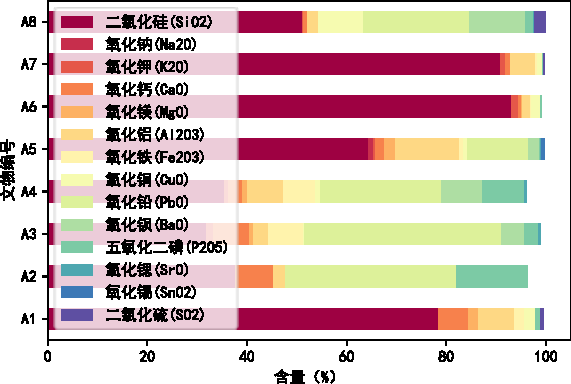
\includegraphics{附件3中不同文物的各个化学成分含量.pdf}
    \caption{附件3中不同文物的各个化学成分含量}
    \label{fig:visual2}
\end{figure}

预测结果中,A2、A3、A4、A5、A8是铅钡类玻璃,A1、A6、A7是高钾类玻璃。结合
图 \ref{fig:all0},可以得知,A1是无风化的高钾类玻璃,A6、A7是风化的高钾
类玻璃,A2、A3、A4是无风化的铅钡类玻璃,A5、A8是风化的铅钡类玻璃。

\subsection{对分类结果的敏感性分析}
\subsubsection{模型求解}
我们假定在无扰动因子下预测出的结果为标准结果A,其中含有八个文物的预测类别:
\[
    A=[a^{(1)},a^{(2)},\dots,a^{(8)}]
\]

在单元素敏感性分析法中,保持文物 $i$ 的其他化学成分的
含量不变,对化学成分 $m$ 添加扰动因子:
\[
    \widetilde{p}_{i,m}=\max(p_{i,m}+\Delta_q, 0) 
\]

其中,$i=A1,A2,...,A8, m=\mathrm{SiO_2,Na_2O,...,SO_2}$,$\Delta_q$ 为
指定范围的扰动因子,当指定范围为 $q$ 时,扰动因子为 $(-q,q]$ 之中的随机数。
由于随机数的添加可能会导致扰动后的含量小于 0,不符合实际,因此要在 0 和实际
扰动含量中取最大值。

对于每个文物 $i$,我们在对化学成分 $m$ 添加指定范围的扰动后,进行 100 次的
预测,统计每一次的预测结果正确率 $K$,对这 100 次的正确率进行统计,分别得到
最小正确率、平均正确率、最大正确率。
\[
    K=1-\frac{\sum_{j=1}^8|a^{(j)}-f(\widetilde{p}_{i,m})^{(j)}|}{8}
\]

在多元素敏感性分析法中,我们通过控制变量法,对文物i的所有化学成分的含量随机
添加扰动因子:
\[
    \widetilde{p}_{i,m}=\max(p_{i,m}+\Delta_{q,m}, 0)
\]

其中,$i=A1,A2,...,A8,m=\mathrm{SiO_2,Na_2O,...,SO_2}$,$\Delta_{q,m}$
为指定范围的扰动因子,当指定范围为 $q$ 时,扰动因子为 $(-q,q]$ 之中的随机
数。由于随机数的添加可能会导致扰动后的含量小于 0,不符合实际,因此要在 0 和
实际扰动含量中取最大值。

对于每个文物 $i$,我们在对所有化学成分添加指定范围的扰动后,进行 100 次的
预测,同样统计每一次的预测结果正确率 $K$,对这 100 次的正确率进行统计,分
别得到最小正确率、平均正确率、最大正确率。

\subsubsection{结论分析}
最终我们得到单元素敏感性分析的变化如图 \ref{fig:PbOSensitivity}、
\ref{fig:other13kindsSensitivity}。
\begin{figure}[!htb]
    \centering
    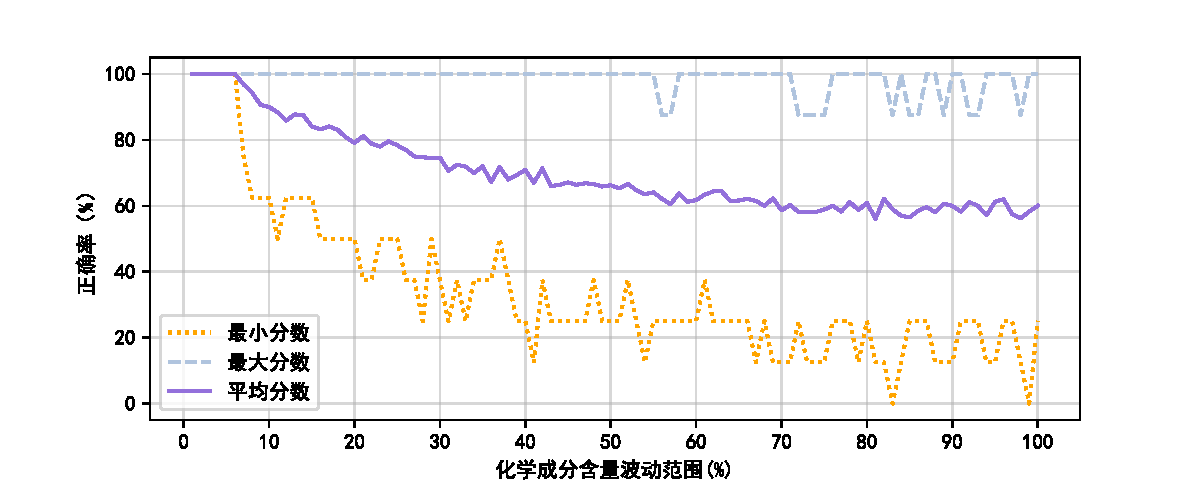
\includegraphics[scale=0.75]{氧化铅(PbO)敏感性分析.pdf}
    \caption{氧化铅(PbO)敏感性分析}
    \label{fig:PbOSensitivity}
\end{figure}
\begin{figure}[!htb]
    \centering
    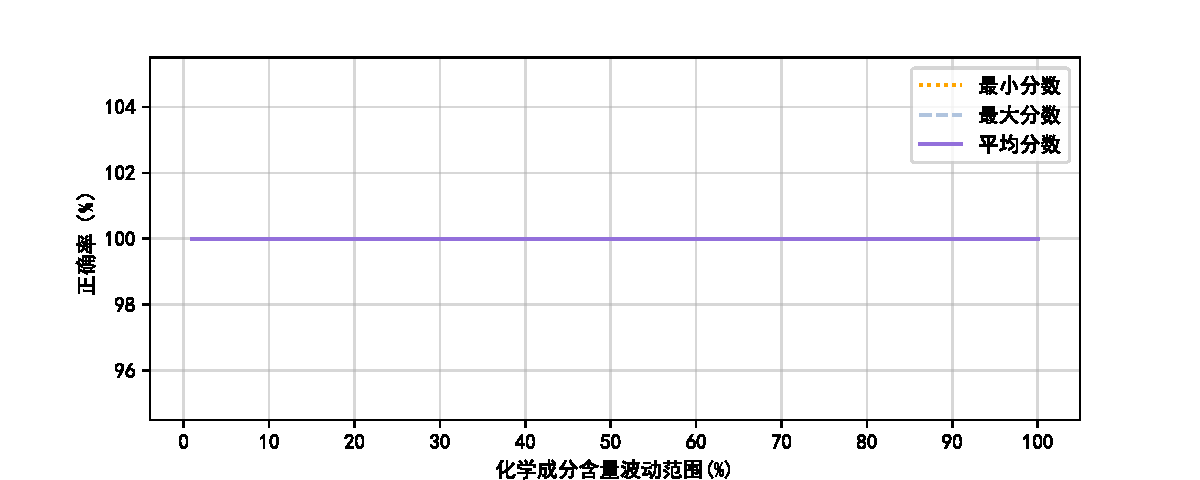
\includegraphics[scale=0.75]{其他13种化学成分含量单元素敏感性分析.pdf}
    \caption{其他13种化学成分含量单元素敏感性分析}
    \label{fig:other13kindsSensitivity}
\end{figure}

可以发现,模型对于氧化铅的化学成分含量波动较为敏感,在波动范围大于 5\% 时初
次出现最小分数低于 100\% 的情况,说明模型开始不准确,在波动范围大于 18\% 时
模型的正确率跌破 50\%,模型预测性能接近失效。此外,其余 13 种化学成分含量的
单元素敏感性分析均表示,模型的准确率受其他化学成分含量的波动影响很小。这与问
题二中我们分析出的玻璃类型与各成分规律相对应。

我们在多元素分析法中最开始添加了所有元素,试图通过波动元素数量的减少将正确率
变化逐步逼近到单元素分析法中的变化。但是全部元素都添加波动因子后,正确率的变
化仍然以 5\% 为临界点,如图 \ref{fig:globalError}、图 \ref{fig:initialError}。
\begin{figure}[!htb]
    \centering
    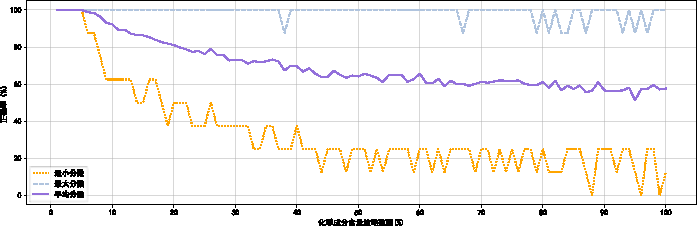
\includegraphics{敏感性分析:全局误差.pdf}
    \caption{敏感性分析:全局误差}
    \label{fig:globalError}
\end{figure}
\begin{figure}[!htb]
    \centering
    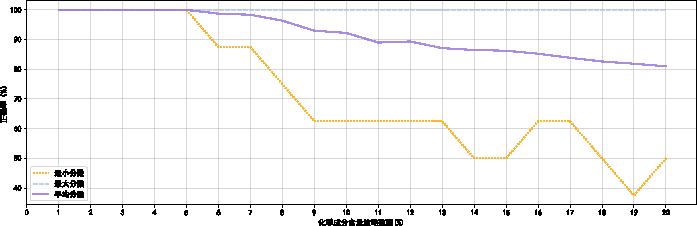
\includegraphics{敏感性分析:开始出现误差.pdf}
    \caption{敏感性分析:开始出现误差}
    \label{fig:initialError}
\end{figure}

我们认为,氧化铅的影响因子过高,导致其他成分的波动与模型的准确率关联较小,因
此全部进行波动因子的添加后,氧化铅带来的影响明显超过了其他成分,占据主导地位,
多元素分析法中得到的图与氧化铅化学元素含量单元素分析法中得到的图大体一致。

考虑到模型并没有使用风化与否这一特征,由于限定了风化条件的含量比例模型在各个
化学成分的范围会进一步缩小,因此如果添加进去,可能会导致整体敏感性升高,氧化
铅含量的敏感性降低,其他化学成分含量的敏感性升高,但是由于现阶段已经得到测试
集正确率为 100\%,模型的准确性能并不会得到提升。

\subsection{不同类别玻璃文物样品的化学成分关联模型}\label{sec:associationModel}%4.1
\subsubsection{模型建立}
设系统行为有多个因子,对应于从 $\mathrm{SiO_2}$ 到 $\mathrm{SO_2}$ 的所有
化学成分,不妨设因子集为 $X=\{x_i |i=1,2,\dots,l\}$,其中 $l$ 为化学成分
种类,共十四种。

由于因素数列 $x_i$ 满足下列条件:
\begin{enumerate}
    \item 数列 $x_i$ 的数据 $x_i(k)$ 之间具有数值可比性,即指定 $x_i(k)$ 与
    $x_j(t)$ 之间的数值是可以比较的,或相等、或接近、或同数量级等;
    \item 数列 $x_i$ 之间具有可接近性,即非平等性;
    \item 数列 $x_i$ 之间具有同级性,即同为适中极性。
\end{enumerate}

故可称 $X$ 为灰关联因子集:

以灰关联因子集 $X$ 中的一个因子 $x_i(1\leqslant i\leqslant l)$ 为参考
数列 $x_i$:
\[
    x_i=\{x_i(k)|k=1,2,\dots,n\}=(x_i(1),x_i(2),\dots,x_i(n)) 
\]
\indent 其中,$n$ 是数据清洗后采样点的数量,共67个。

对于相关因素 $x_i\in X\quad(1\leqslant i\leqslant l)$,即比较数列为:
\[
    x_j={x_j(k)|k=1,2,\dots,n}=(x_j(1),x_j(2),\dots,x_j(n))\quad (j=1,2,\dots,l)
\]

则行为因子参考数列 $x_i$ 和相关因素比较数列 $x_j$ 二者间的绝对差为:
\[
    \Delta_{ij}(k)=|x_i(k)-x_j(k)|\quad (k=1,2,\dots,n;j=1,2,\dots,l)
\]

相应的差数列为 $\Delta_{ij}=(\Delta_{ij}(1),\Delta_{ij}(2),\dots,
\Delta_{ij}(n))$,其比较数列 $x_j$ 对参考数列 $x_i$ 在第 $k$ 点的灰关联为:
\[
    r(x_i(k),x_j(k))=\frac{\displaystyle\min_i\min_j\min_k\Delta_{ij}(k) +
     \alpha\max_i\max_j\max_k\Delta_{ij}(k)}{\displaystyle\Delta_{ij}(k) +
     \alpha\max_i\max_j\max_k\Delta_{ij}(k)}
\]
\indent 其中常数 $\alpha\in[0,1]$ 为分辨率系数。

于是有 $x_j$ 对 $x_i$ 的灰关联度为:
\begin{equation}
    r_{ij}=r(x_i,x_j)=\frac{1}{n}\sum_{k=1}^nr(x_i(k),x_j(k))\quad
    (i=1,2,\dots,m;j=1,2,\dots,l)
    \label{eq:4-0}
\end{equation}

\subsubsection{模型求解}
将数据依照高钾和铅钡玻璃类型进行分类,并将分类后的数据进行清洗,剔除掉不符合含
量范围的两个采样点,填充空白数据为 0。

对于高钾类型玻璃,依次对于每个化学成分,提取其在所有采样点的含量作为标准因素数
列 $x_i$ ,并使用公式 \eqref{eq:4-0} 求得所有成分 $x_j$ 对 $x_i$ 的灰色关
联度 $r_{ij}$ ,其中 $j=1,2,\dots,l$。

以第 $i$ 行中第 $j$ 列表示灰色关联度 $r_{ij}$,将求解结果呈现在矩阵中如图
\ref{fig:HighKgrey}。
\begin{figure}[!htb]
    \centering
    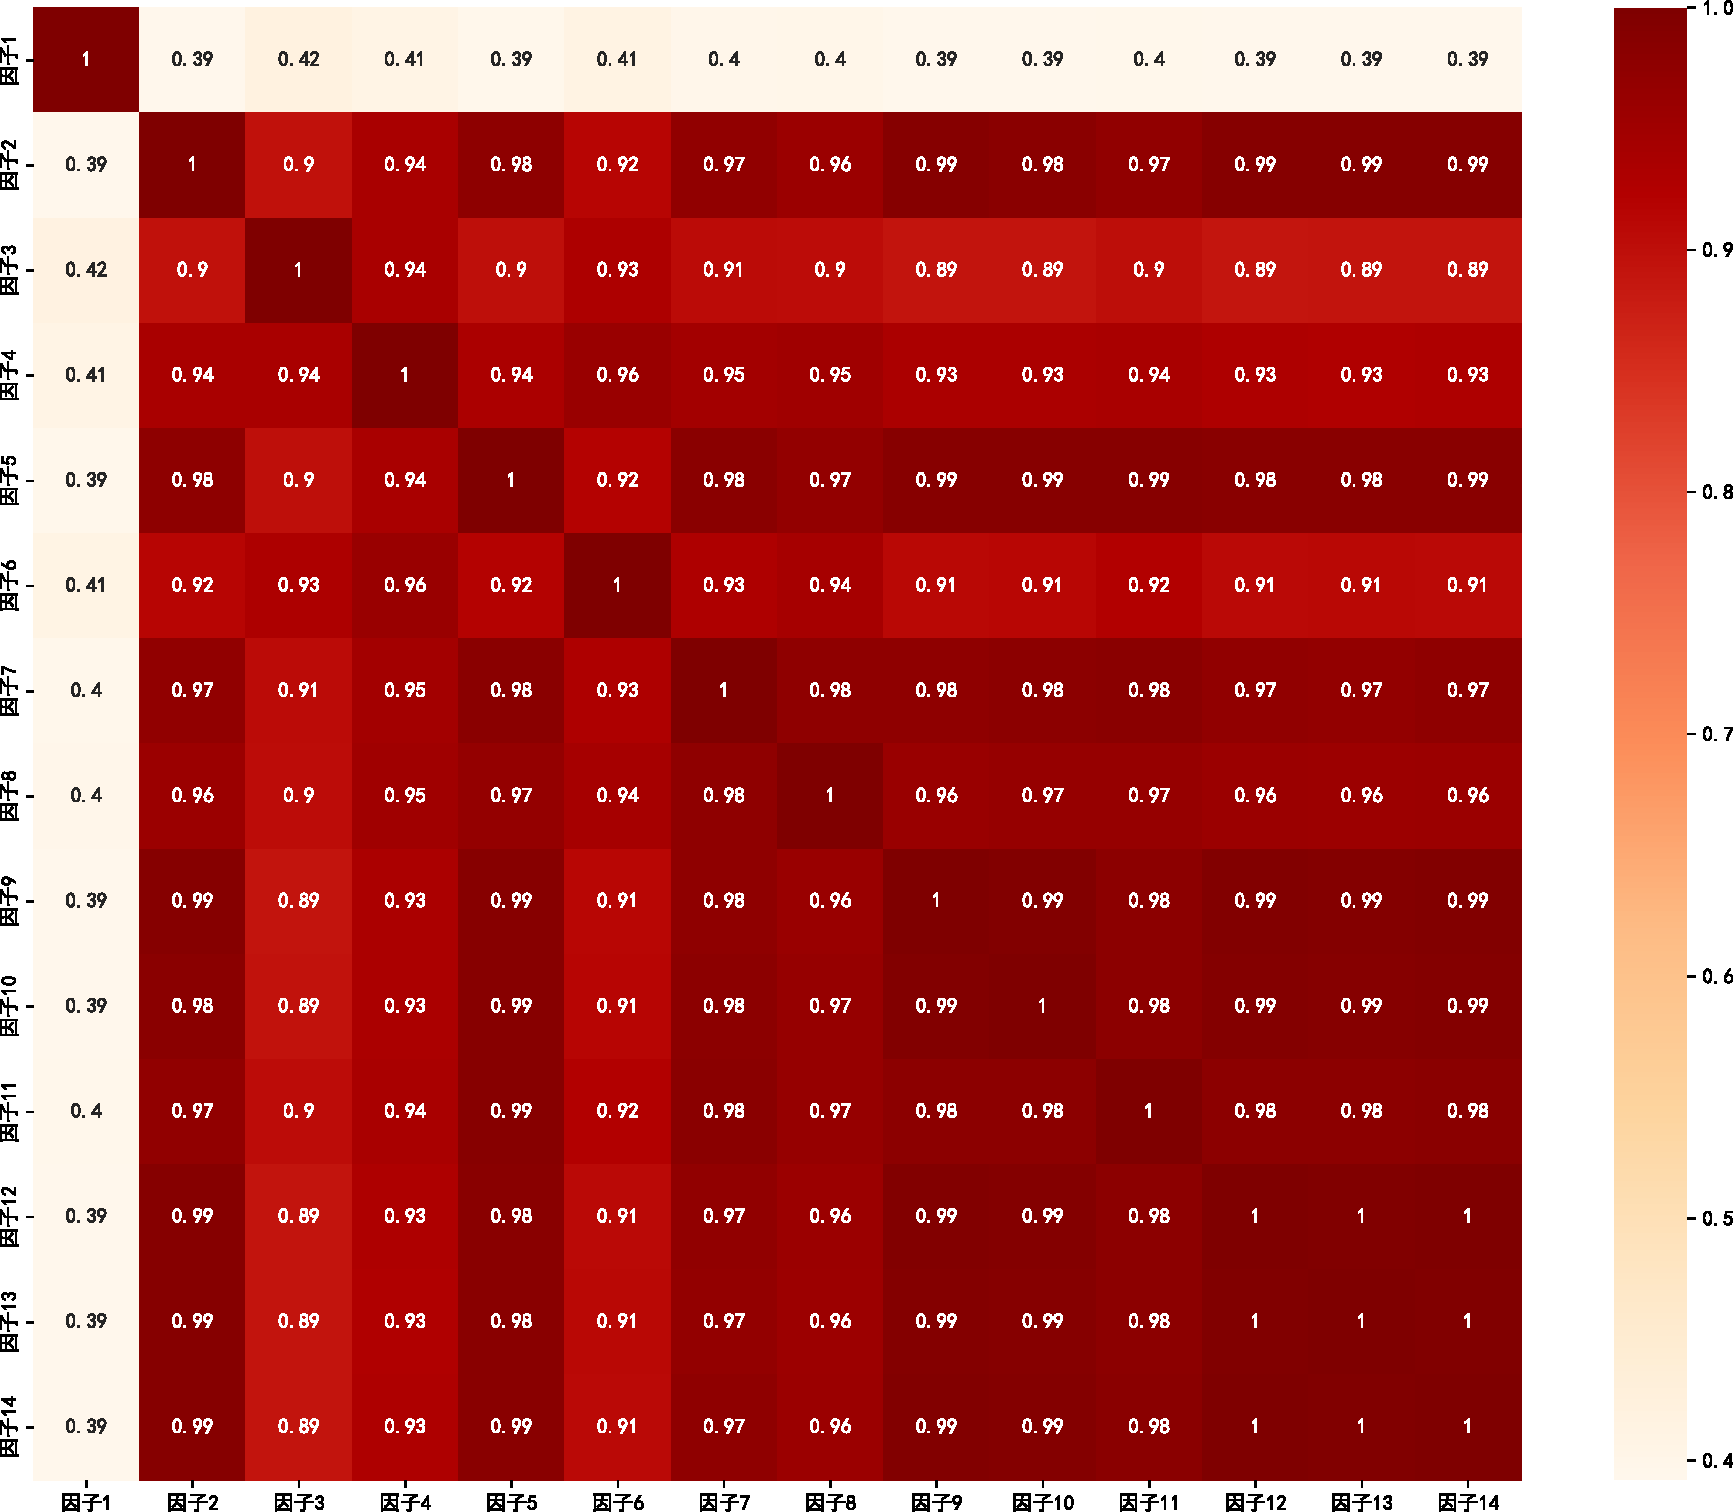
\includegraphics[scale=0.25]{高钾玻璃各成分灰色关联热力图.pdf}
    \caption{高钾玻璃各成分灰色关联热力图}
    \label{fig:HighKgrey}
\end{figure}

相似地,对于铅钡类型玻璃,以第 $i$ 行中第 $j$ 列表示灰色关联度 $r_{ij}$,将求解
结果呈现在矩阵中如图 \ref{fig:PbBagrey}。
\begin{figure}[!htb]
    \centering
    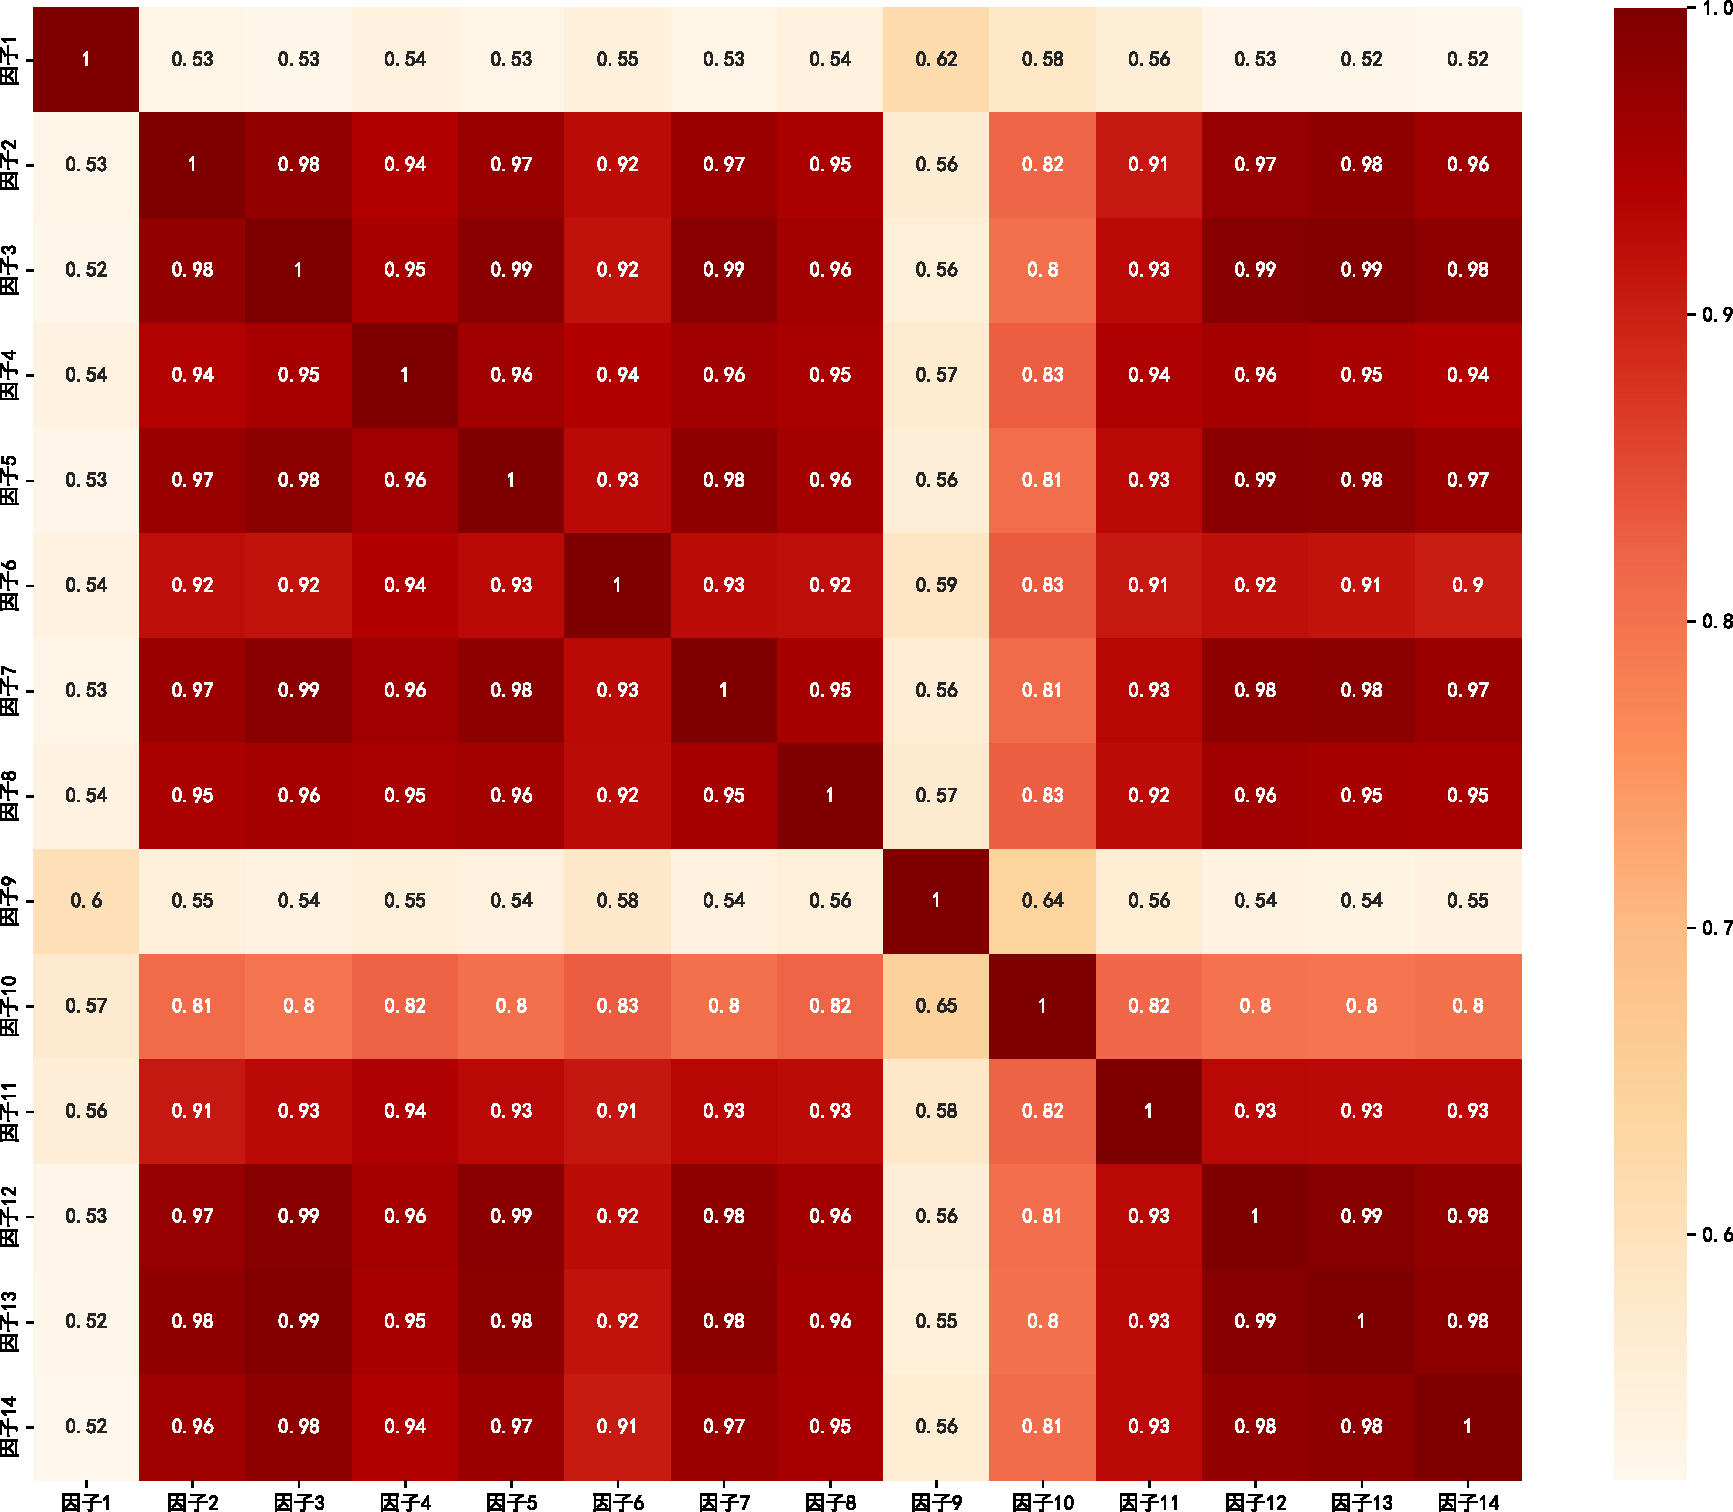
\includegraphics[scale=0.25]{铅钡玻璃各成分灰色关联热力图.pdf}
    \caption{铅钡玻璃各成分灰色关联热力图}
    \label{fig:PbBagrey}
\end{figure}

其中,因子 1、因子 2、因子 3、因子 4、因子 5、因子 6、因子 7、因子 8、
因子 9、因子 10、因子 11、因子 12、因子 13、因子 14,分别对应于化学成分:
二氧化硅($\mathrm{SiO_2}$)、氧化钠($\mathrm{Na_2O}$)、氧化钾($\mathrm{K_2O}$)、
氧化钙($\mathrm{CaO}$)、氧化镁($\mathrm{MgO}$)、氧化铝($\mathrm{Al_2O_3}$)、
氧化铁($\mathrm{Fe_2O_3}$)、氧化铜($\mathrm{CuO}$)、氧化铅(PbO)、
氧化钡(BaO)、五氧化二磷($\mathrm{P_2O_5}$)、氧化锶(SrO)、
氧化锡($\mathrm{SnO_2}$)、二氧化硫($\mathrm{SO_2}$)。

\subsubsection{结果分析}
在高钾类型玻璃中,可以看出,二氧化硅($\mathrm{SiO_2}$)与其他化学成分的关联度都
相差不大且并不高,没有明显的规律。其他因素的灰色关联度均不低于 0.89,显示出较强
的关联性。

在除去二氧化硅($\mathrm{SiO_2}$)之外,氧化钠($\mathrm{Na_2O}$)与其他化学成分
的关联较明显;氧化镁(MgO)与氧化铁($\mathrm{Fe_2O_3}$)、氧化铜(CuO)、氧化铅(PbO)、
氧化钡(BaO)、五氧化二磷($\mathrm{P_2O_5}$)、氧化锶(SrO)、氧化锡($\mathrm{SnO_2}$)、
二氧化硫($\mathrm{SO_2}$)的关联较明显;氧化铁($\mathrm{Fe_2O_3}$)、氧化铜(CuO)、
氧化铅(PbO)、氧化钡(BaO)、五氧化二磷($\mathrm{P_2O_5}$)、氧化锶(SrO)、
氧化锡($\mathrm{SnO_2}$)、二氧化硫($\mathrm{SO_2}$)相互之间的关联性较为明
显;而在氧化锶(SrO)、氧化锡($\mathrm{SnO_2}$)、二氧化硫($\mathrm{SO_2}$)中,
彼此之间具有极强的关联性。同时也可以看出,当一个化学成分受其他化学成分影响大时,
该成分也会对影响它的化学成分具有较大的影响。

在铅钡类型玻璃中,可以看出,二氧化硅($\mathrm{SiO_2}$)、氧化铅(PbO)与其他化
学成分的关联度都相差不大且并不高,没有明显的规律,但二者之间具有一定的联系,与
氧化钡(BaO)彼此的关联度也相对其他成分较高。

在所有化学成分除去二者之外,氧化钡(BaO)与其他成分的关联度比之二氧化硅
($\mathrm{SiO_2}$)、氧化铅(PbO)较高,但也低于 0.9。氧化铝($\mathrm{Al_2O_3}$)、
五氧化二磷($\mathrm{P_2O_5}$)与其他化学成分的灰色关联度高于氧化钡(BaO)但低
于氧化钙(CaO)、氧化铜(CuO)。其余化学成分的彼此关联度都较高。

\subsection{化学成分关联模型差异性分析}
在 \ref{sec:associationModel} 节中,本文建立的化学成分关联模型是以矩阵形式
表现的。在此,我们对矩阵形式的关联模型进行差异性分析。

对于不同玻璃类型下的灰色关联系数矩阵 $R_{\text{高钾}}$ 和 $R_{\text{铅钡}}$,
我们分别进行了关联系数平均值、方差、最小值、最大值的统计:
\begin{gather*}
    \mathrm{avg}=\frac{\sum_{i=1}^{14}\sum_{j=1}^{14}r_{ij}}
    {14\times 14} \\
    \mathrm{var}=\sum_{i=1}^{14}\sum_{j=1}^{14}(r_{ij}-\mathrm{avg})^2 \\
    R\min = \min_i\min_jr_{ij} \\
    R\max = \max_i\max_jr_{ij}
\end{gather*}

得到 $\mathrm{avg}_{\text{高钾}}=0.8841977189171356$,
$\mathrm{avg}_{\text{铅钡}}=0.8388290737388091$,
$var_{\text{高钾}}=0.037$ $173578025678645$,$var_{\text{铅钡}}=0.03063280766634742$,
$R\min_{\text{高钾}}=0.3919661616394346$,$R\min_{\text{铅钡}}=0.5200093293479898$,
$R\max_{\text{高钾}}=1$,$R\max_{\text{铅钡}}=1$。可以发现,整体上高钾类型的内部规律比
铅钡类型强,同时内部不同成分之间关联系数的差别更大。相比起铅钡玻璃,高钾玻璃存在更加细微而
较弱的内部关联。

由于上一小问总得到的矩阵均为 $14\times 14$ 的矩阵,第 $i$ 行的第 $j$ 列表示
灰色关联系数 $r_{ij}$,我们首先将高钾类型玻璃的各成分关联矩阵与铅钡类型玻璃的
各成分关联矩阵相减,得到关联性差异矩阵 $R_{\mathrm{diff}}$:
\[
    R_{\mathrm{diff}}=R_{\text{高钾}}-R_{\text{铅钡}}
\]

将 $R_{\mathrm{diff}}$ 进行热力图可视化后,如图 \ref{fig:diff} 所示。
\begin{figure}[!htb]
    \centering
    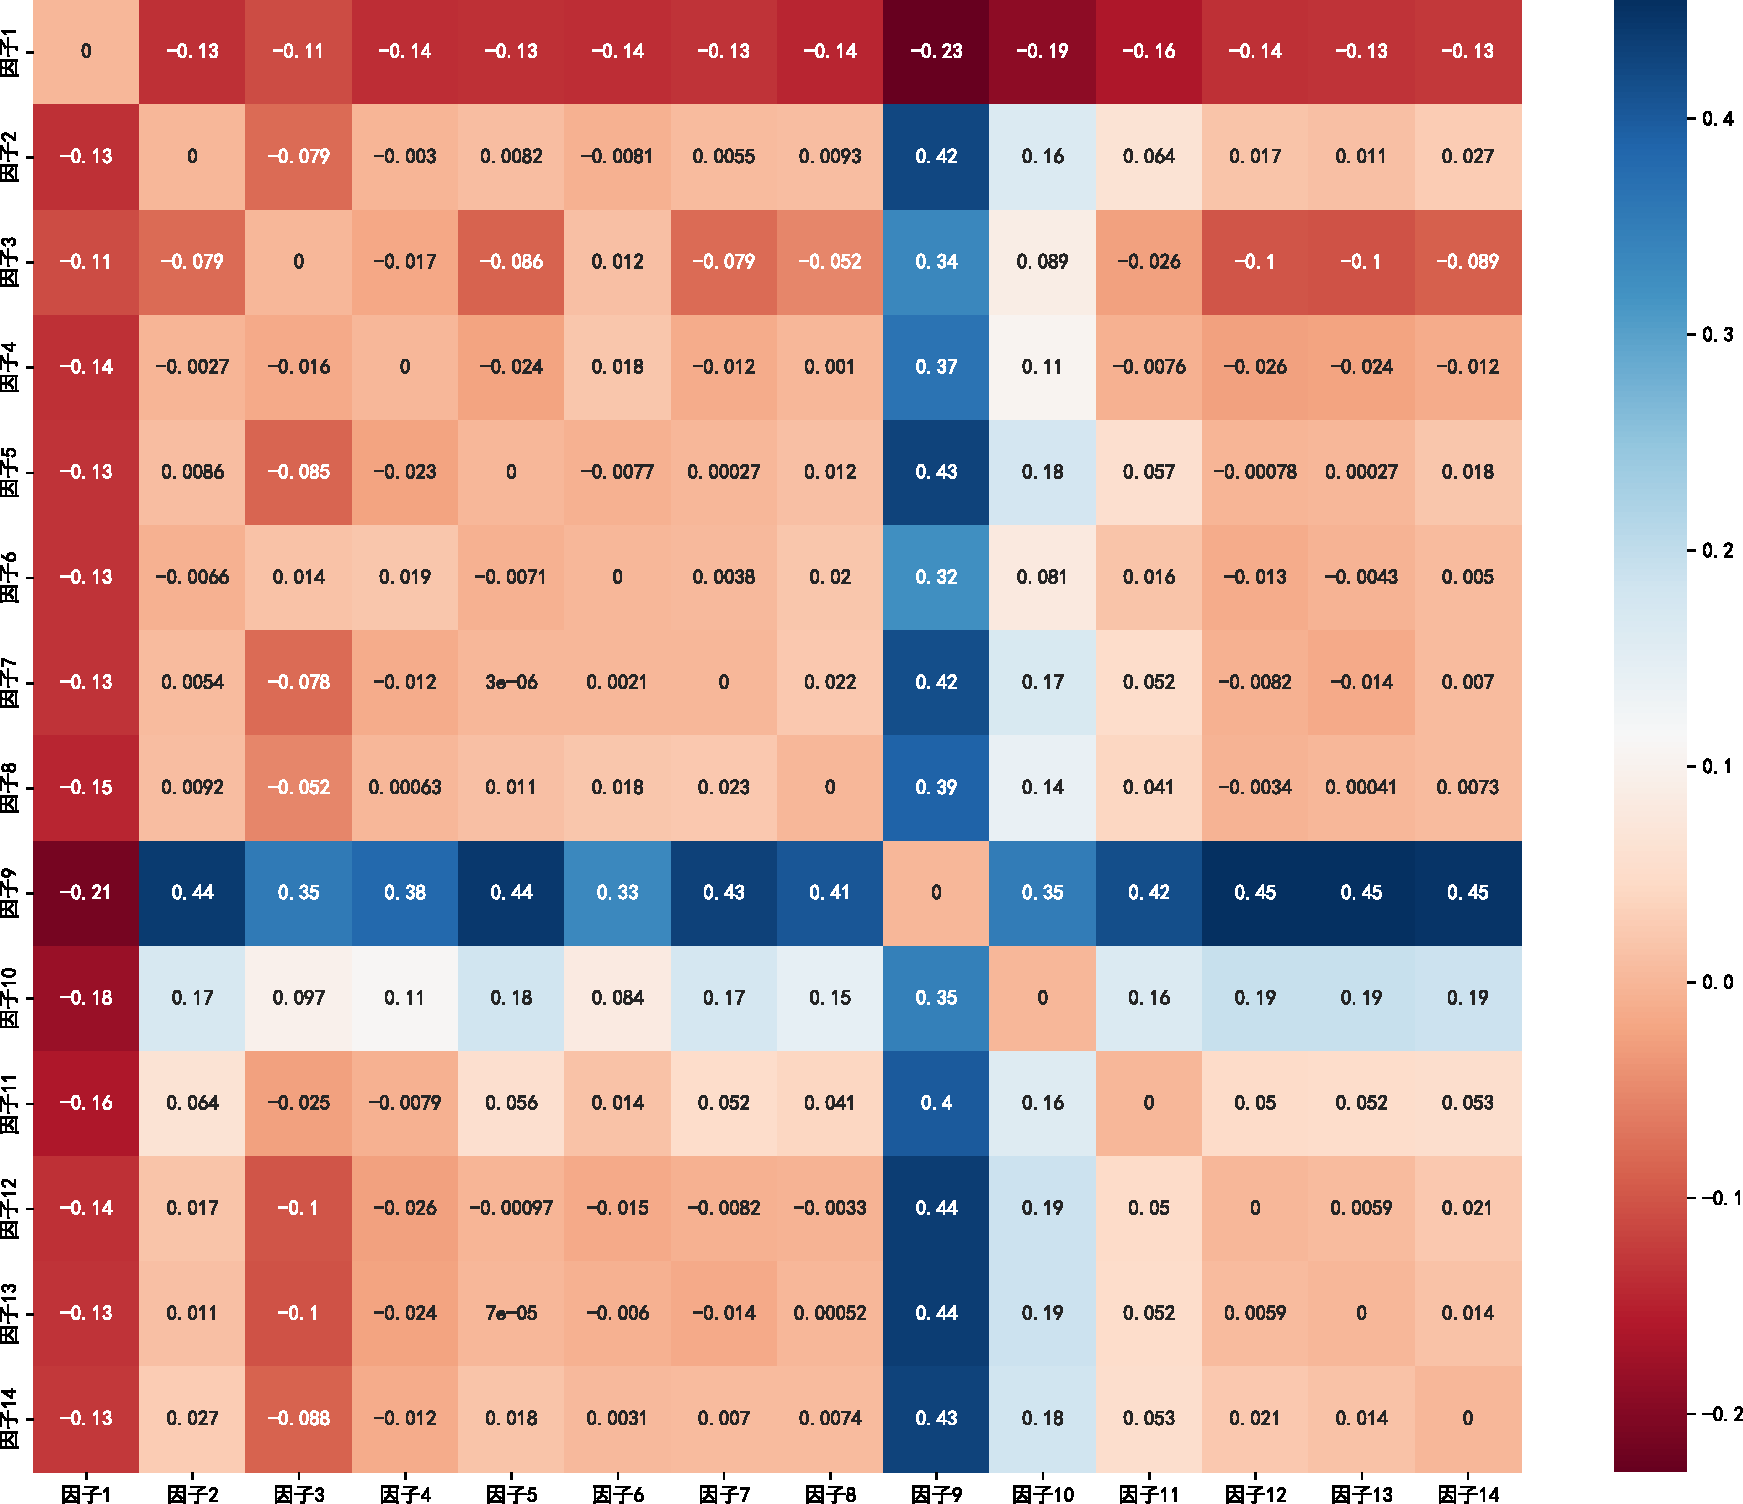
\includegraphics[scale=0.25]{不同玻璃各成分灰色关联变动热力图.pdf}
    \caption{不同玻璃各成分灰色关联变动热力图}
    \label{fig:diff}
\end{figure}

从图中可以看出,两种玻璃的内部化学成分之间的关联关系主要在二氧化硅($\mathrm{SiO_2}$)
和氧化铅(PbO)中差异较明显。高钾玻璃中氧化铅(PbO)、氧化钡(BaO)和其他化学成
分的关联相比铅钡玻璃中更加明显,铅钡玻璃中除去氧化铅(PbO)、氧化钡(BaO)之外
的化学成分,尤其是二氧化硅($\mathrm{SiO_2}$)、氧化钾($\mathrm{K_2O}$)和
其他化学成分的关联相比高钾玻璃中更加明显。此外,氧化钾($\mathrm{K_2O}$)和
氧化钠($\mathrm{Na_2O}$)的关联在高钾玻璃中也明显弱于在铅钡玻璃中。其余因素
的关联性差异则并不那么明显,整体上而言,关联性差异值绝对值的平均值为0.1000910944651129。

除掉直接相减之外,
对于普通的一维、二维向量,有较为直接的方法进行比较。但是对于高阶的矩阵,并没有
一个直接的方法来进行比较。所以需要选取一种方法来对矩阵进行度量。本文选择对矩阵
计算范数来进行度量。衡量矩阵的距离远近本质上就是矩阵差的范数,因此使用 
$R_{\mathrm{diff}}$ 来进一步确认两个矩阵之间的关联性差异性。

为了提高可靠性。本文选择了多个矩阵范数进行比较。在此,我们选择常用的 
1-范数、2-范数和 $\infty$-范数来分布度量矩阵。

矩阵的 1-范数为:
\[
    \|R\|_1 = \max_{1\leqslant j\leqslant n}\sum_{i=1}^n|r_{ij}|
\]
\indent 表示的意义为 $R$ 的每列绝对值之和的最大值,又被称为 $R$ 的列范数。

矩阵的 2-范数为:
\[
    \|R\|_2 = \sqrt{\lambda_{\max}(R^TR)}
\]
\indent 被称为 $R$ 的 2-范数,其中 $\lambda_{\max}(R^TR)$ 为 $R^TR$ 的特征
值的绝对值的最大值。

矩阵的 $\infty$-范数为:
\[
    \|R\|_\infty = \max_{1\leqslant i\leqslant n}\sum_{j=1}^n|r_{ij}|
\]
\indent 表示的意义为 $R$ 的每行绝对值之和的最大值,又被称为 $R$ 的行范数。

最终得到关联性差值矩阵的第一范数、第二范数、无穷范数分别为:$4.96552426311$ $2795$,
 1.753305500203036,5.128146207785363;而高钾玻璃关联性矩阵的第一范数、第二
 范数、无穷范数分别为:12.995063902829889,12.639204977558006,
 12.99708630682788;铅钡玻璃的关联性矩阵的第一范数、第二范数、无穷范数分别
 为:12.535448433000091,11.946637357116344,12.562524663091839。可以得知,
 两个玻璃化学成分系统的规律差异值约占原始值的三成。

 \section{模型的不足}
 在问题三中鉴别文物的类型时,对于其中的化学成分含量并没有考虑风化与否的因素。
 这会导致模型鉴别风化程度较高的文物产生的结果与实际情况会有一定的偏差。除此外,
 模型对于化学成分 PbO 波动的敏感性较大,当其波动范围大于 18\% 时,模型的正确
 率就已低于 50\%。

\begin{thebibliography}{9}
    \bibitem{ref1}李青会,黄教珍,李飞,干福熹.中国出土的一批战国古玻璃样品化学成分的检测[J].文物保护与考古科学,2006,(02):8-13.
    \bibitem{ref2}李青会,周虹志,黄教珍,干福熹,张平.一批中国古代镶嵌玻璃珠化学成分的检测报告[J].江汉考古,2005,(04):79-86+93.
\end{thebibliography}

\begin{appendices}
\section{问题 1 表面风化与纹饰、类型、颜色分析的卡方检验代码}
\begin{lstlisting}[language=Python]
import pandas as pd 
from  scipy.stats import chi2_contingency
import numpy as np
import matplotlib.pyplot as plt
%matplotlib inline %config InlineBackend.figure_format = 'svg'

df_if_slak = pd.read_excel("附件.xlsx",sheet_name="表单1")
df_if_slak = df_if_slak.drop(14, axis=0)
df_if_slak = df_if_slak.drop(16, axis=0)
df_if_slak.columns = ['num', 'grain', 'type', 'color', 'weathering']

#取出风化和无风化的两类
df_yes = df_if_slak[df_if_slak['weathering'].isin(['风化'])]
df_no = df_if_slak[df_if_slak['weathering'].isin(['无风化'])]
print(df_yes,'\n', df_no)
#4个颜色缺失,

#对风化的一类进行进一步统计:玻璃类型,纹饰,颜色
df_yes_type = df_yes.type.value_counts() #玻璃类型
df_yes_grain = df_yes.grain.value_counts() #纹饰
df_yes_color = df_yes.color.value_counts() #颜色
print(df_yes_type, '\n', df_yes_grain, '\n', df_yes_color)#34 34 30

#对无风化的一类进行进一步统计:玻璃类型,纹饰,颜色
df_no_type = df_no.type.value_counts() #玻璃类型
df_no_grain = df_no.grain.value_counts() #纹饰
df_no_color = df_no.color.value_counts() #颜色
print(df_no_type, '\n', df_no_grain, '\n', df_no_color)#22 22 22

#玻璃类型
'''
type   铅钡   高钾
yes    28      6
no     12      10
'''
kf_data = np.array([[28, 6], [12, 10]])
kf = chi2_contingency(kf_data)
print('chisq-statistic=%.4f, p-value=%.4f, df=%i expected_frep=%s'%kf)
#结论: 因为p值=0.0516>0.05, 故不拒绝原假设,无充分证据表明两个因素之间存在关系(接受原假设, 认为玻璃类型和是否风化无显著差别。)

#纹饰
'''
grain   A    B    C
yes     11   6    17
no      11   0    11
'''
kf_data = np.array([[11, 6, 17], [11, 0, 11]])
print(kf_data)
kf = chi2_contingency(kf_data)
print('chisq-statistic=%.4f, p-value=%.4f, df=%i expected_frep=%s'%kf)
#结论: 因为p值=0.0845>0.05, 故不拒绝原假设,无充分证据表明两个因素之间存在关系(接受原假设, 认为玻璃纹饰和是否风化无显著差别。)

#颜色
    
'''浅蓝    12
蓝绿     9
深绿     4
紫      2
黑      2
浅绿     1

蓝绿    6
浅蓝    6
深绿    3
深蓝    2
紫     2
浅绿    2
绿     1

color 蓝绿  浅蓝  深绿  深蓝  紫  浅绿  绿  黑
yes    9     12    4     0    2    1    0   2
no     6     6     3     2    2    2    1   0
'''
kf_data = np.array([[9, 12, 4, 0,2,1,0,2], [6,6,3,2,2,2,1,0]])
print(kf_data)
kf = chi2_contingency(kf_data)
print('chisq-statistic=%.4f, p-value=%.4f, df=%i expected_frep=%s'%kf)
#结论: 因为p值=0.0985>0.05, 故不拒绝原假设,无充分证据表明两个因素之间存在关系(接受原假设, 认为玻璃纹饰和是否风化无显著差别。)
\end{lstlisting}

\section{问题 1 表面风化与纹饰、类型、颜色的斯皮尔曼系数代码}
\begin{lstlisting}[language=Python]
df = pd.DataFrame(df_if_slak)
# df = df.dropna()
df = df.drop('num', axis=1)

df.loc[:,'grain'].replace('A',0,inplace=True)
df.loc[:,'grain'].replace('B',1,inplace=True)
df.loc[:,'grain'].replace('C',2,inplace=True)
df.loc[:,'type'].replace('高钾',0,inplace=True)
df.loc[:,'type'].replace('铅钡',1,inplace=True)
df.loc[:,'color'].replace('黑',-1+1,inplace=True)
df.loc[:,'color'].replace('蓝绿',3+1,inplace=True)
df.loc[:,'color'].replace('浅蓝',2+1,inplace=True)
df.loc[:,'color'].replace('深绿',6+1,inplace=True)
df.loc[:,'color'].replace('深蓝',1+1,inplace=True)
df.loc[:,'color'].replace('紫',0+1,inplace=True)
df.loc[:,'color'].replace('浅绿',4+1,inplace=True)
df.loc[:,'color'].replace('绿',5+1,inplace=True)
df.loc[:,'weathering'].replace('无风化',0,inplace=True)
df.loc[:,'weathering'].replace('风化',1,inplace=True)
df_na = df.corr(method="pearson")

import scipy
scipy.stats.spearmanr(df, b=None, axis=0, nan_policy='propagate')
\end{lstlisting}

\section{问题 1 正态分布检验代码}
\begin{lstlisting}[language=Python]
import pandas as pd 
import matplotlib.pyplot as plt
import numpy as np
from scipy import stats
from  scipy.stats import chi2_contingency
%matplotlib inline %config InlineBackend.figure_format = 'svg'
plt.rcParams['font.sans-serif']=['SimHei']

plt.rcParams['axes.unicode_minus'] = False

df_if = pd.read_excel("附件.xlsx",sheet_name="表单2")
COL_NAME = '表面风化'
nos = [23,25,29,30,44,45,48,54,56,60]
seroius = [10, 27, 62]
for ROW_INT in nos:
    df_if.loc[ROW_INT,COL_NAME] = '无风化'
for ROW_INT in seroius:
    df_if.loc[ROW_INT,COL_NAME] = '严重风化'
df_if    

names = df_if.columns.tolist()
names

df_if = df_if.fillna(0)
df_gaojia = df_if[df_if['类型'].isin(['高钾'])]
df_gaojia_yes = df_gaojia[df_gaojia['表面风化'].isin(['风化'])]
df_gaojia_no = df_gaojia[df_gaojia['表面风化'].isin(['无风化'])]
df_gaojia_ser = df_gaojia[df_gaojia['表面风化'].isin(['严重风化'])]

df_qianbei = df_if[df_if['类型'].isin(['铅钡'])]
df_qianbei_yes = df_qianbei[df_qianbei['表面风化'].isin(['风化'])]
df_qianbei_no = df_qianbei[df_qianbei['表面风化'].isin(['无风化'])]
df_qianbei_ser = df_qianbei[df_qianbei['表面风化'].isin(['严重风化'])]

def Gaussion_exam(df_to_exam, name):
    for i in range(3,len(names)):
        a = np.array(df_to_exam.loc[:,names[i]])
#         print(a)
        print('{}{}K-S检验:{}'.format(name, names[i], stats.kstest(a, 'norm')))

Gaussion_exam(df_gaojia, '高钾类型玻璃')
print()
Gaussion_exam(df_qianbei, '铅钡类型玻璃')
print('\n输出结果中第一个为统计量,第二个为P值(注:统计量越接近0就越表明数据和标准正态
分布拟合的越好,如果P值大于显著性水平,通常是0.05,接受原假设,则判断样本的总体服从正态分布)')
\end{lstlisting}

\section{问题 1 不同玻璃类型下风化化学成分划分规律分析代码}
\begin{lstlisting}[language=Python]
import pandas as pd 
import matplotlib.pyplot as plt
import numpy as np
from scipy import stats
from  scipy.stats import chi2_contingency
%matplotlib inline %config InlineBackend.figure_format = 'svg'
plt.rcParams['font.sans-serif']=['SimHei']

plt.rcParams['axes.unicode_minus'] = False
df_if = pd.read_excel("附件.xlsx",sheet_name="表单2")
COL_NAME = '表面风化'
nos = [23,25,29,30,44,45,48,54,56,60]
seroius = [10, 27, 62]
for ROW_INT in nos:
    df_if.loc[ROW_INT,COL_NAME] = '无风化'
for ROW_INT in seroius:
    df_if.loc[ROW_INT,COL_NAME] = '严重风化'
df_if    
names = df_if.columns.tolist()
names
df_if = df_if.fillna(0)
df_gaojia = df_if[df_if['类型'].isin(['高钾'])]
df_gaojia_yes = df_gaojia[df_gaojia['表面风化'].isin(['风化'])]
df_gaojia_no = df_gaojia[df_gaojia['表面风化'].isin(['无风化'])]
df_gaojia_ser = df_gaojia[df_gaojia['表面风化'].isin(['严重风化'])]

df_qianbei = df_if[df_if['类型'].isin(['铅钡'])]
df_qianbei_yes = df_qianbei[df_qianbei['表面风化'].isin(['风化'])]
df_qianbei_no = df_qianbei[df_qianbei['表面风化'].isin(['无风化'])]
df_qianbei_ser = df_qianbei[df_qianbei['表面风化'].isin(['严重风化'])]

df_gaojia_data = pd.DataFrame()
df_gaojia_data['无风化最小值'] = df_gaojia_no.loc[:,names[3:]].min()
df_gaojia_data['无风化最大值'] = df_gaojia_no.loc[:,names[3:]].max()
df_gaojia_data['风化最小值'] = df_gaojia_yes.loc[:,names[3:]].min()
df_gaojia_data['风化最大值'] = df_gaojia_yes.loc[:,names[3:]].max()
df_gaojia_data['严重风化最小值'] = df_gaojia_ser.loc[:,names[3:]].min()
df_gaojia_data['严重无风化最大值'] = df_gaojia_ser.loc[:,names[3:]].max()
df_gaojia_data.to_csv('高钾类型各含量范围数据统计.csv')

df_qianbei_data = pd.DataFrame()
df_qianbei_data['无风化最小值'] = df_qianbei_no.loc[:,names[3:]].min()
df_qianbei_data['无风化最大值'] = df_qianbei_no.loc[:,names[3:]].max()
df_qianbei_data['风化最小值'] = df_qianbei_yes.loc[:,names[3:]].min()
df_qianbei_data['风化最大值'] = df_qianbei_yes.loc[:,names[3:]].max()
df_qianbei_data['严重风化最小值'] = df_qianbei_ser.loc[:,names[3:]].min()
df_qianbei_data['严重无风化最大值'] = df_qianbei_ser.loc[:,names[3:]].max()
df_qianbei_data.to_csv('铅钡类型各含量范围数据统计.csv')
\end{lstlisting}

\section{问题 1 高钾风化还原预测代码}
\begin{lstlisting}[language=Python]
import pandas as pd 
import matplotlib.pyplot as plt
import numpy as np
from scipy import stats
from  scipy.stats import chi2_contingency
%matplotlib inline %config InlineBackend.figure_format = 'svg'
plt.rcParams['font.sans-serif']=['SimHei']

plt.rcParams['axes.unicode_minus'] = False

df_if = pd.read_excel("附件.xlsx",sheet_name="表单2")
COL_NAME = '表面风化'
nos = [23,25,29,30,44,45,48,54,56,60]
seroius = [10, 27, 62]
for ROW_INT in nos:
    df_if.loc[ROW_INT,COL_NAME] = '无风化'
for ROW_INT in seroius:
    df_if.loc[ROW_INT,COL_NAME] = '严重风化'
df_if    

names = df_if.columns.tolist()
names

df_if = df_if.fillna(0)
df_if = df_if[df_if['类型'].isin(['高钾'])]
df_if

df_if.loc[:,'表面风化'].replace('无风化',0,inplace=True)
df_if.loc[:,'表面风化'].replace('风化',1,inplace=True)
df_if.loc[:,'表面风化'].replace('严重风化',2,inplace=True)
names = df_if.columns.tolist()[3:]
print(names)
df_if

df_yes = df_if[df_if['表面风化'].isin([1])]
df_no = df_if[df_if['表面风化'].isin([0])]
df_ser = df_if[df_if['表面风化'].isin([2])]
print(df_ser)

yes_min1 = dict()
yes_max1 = dict()
no_min1 = dict()
no_max1 = dict()
yes_mean1 = dict()
no_mean1 = dict()

for name in names:
    yes_min1[name] = [df_yes[name].min()]
    yes_max1[name] = [df_yes[name].max()]
    yes_mean1[name] = [df_yes[name].mean()]
    no_min1[name] = [df_no[name].min()]
    no_max1[name] = [df_no[name].max()]
    no_mean1[name] = [df_no[name].mean()]
l = []
dicts1 = [no_min1, no_mean1, no_max1]
dicts2 = [yes_min1, yes_mean1, yes_max1]
for i in range(3):
    dic1 = dicts1[i]
    dic2 = dicts2[i]
    df_tmp1 = pd.DataFrame.from_dict(dic1)
    df_tmp2 = pd.DataFrame.from_dict(dic2)
    df_tmp = pd.concat([df_tmp1, df_tmp2])
    df_tmp.index = ['无风化', '一般风化']
    l.append(df_tmp)
cm='Spectral'   
num = 0
pic_names = ['高钾玻璃含量最小值一般风化前后对比', '高钾玻璃含量平均值一般风化前后对比', '高钾玻璃含量最大值一般风化前后对比']
for dff in l:
    print(dff, '\n\n', dff.diff())
    dff.plot(kind='bar', cmap=cm, figsize=(10,5))
    plt.legend(loc='center')
    plt.rcParams['font.sans-serif']=['SimHei']
    plt.rcParams['axes.unicode_minus'] = False
    plt.xticks(rotation=0)
    plt.xlabel('采样点风化程度')
    plt.ylabel('各化学成分含量(%)')
    plt.savefig('%s.svg'%pic_names[num])
    plt.show()
    num += 1

df_diff = l[1].diff()
df_diff.to_csv('高钾玻璃一般后-前.csv')

df_tmp = l[1]
df_quotient = pd.DataFrame(df_tmp.T[df_tmp.index [0]] / (df_tmp.T [df_tmp.index [-1]] + 1e-9))
df_quotient.T.to_csv('高钾玻璃一般前除以后.csv')
print(df_quotient)

df_diff = pd.read_csv('高钾玻璃一般后-前.csv', encoding='gbk')
a_d = df_diff.values[0]

# print(df_49_1,'\n', df_diff.T, '\n', df_49_0)
def array_no(weathered):
    a1 = weathered.T.values[0]
#     print(a1, a_d)
    a0_compute1 = a1 - a_d
    return a0_compute1

l = []
df_yes.to_csv('高钾玻璃yes_tmp.csv')
df_yes1 = df_yes[names]
for i in df_yes.index:
    l.append(array_no(pd.DataFrame(df_yes1.loc[i, :])))
ans = pd.DataFrame(l)

ans.to_csv('高钾玻璃yes_tmp2.csv')
\end{lstlisting}

\section{问题 1 铅钡风化还原预测代码}
\begin{lstlisting}[language=Python]
import pandas as pd 
import matplotlib.pyplot as plt
import numpy as np
from scipy import stats
from  scipy.stats import chi2_contingency
%matplotlib inline %config InlineBackend.figure_format = 'svg'
plt.rcParams['font.sans-serif']=['SimHei']

plt.rcParams['axes.unicode_minus'] = False

df_if = pd.read_excel("附件.xlsx",sheet_name="表单2")
COL_NAME = '表面风化'
nos = [23,25,29,30,44,45,48,54,56,60]
seroius = [10, 27, 62]
for ROW_INT in nos:
    df_if.loc[ROW_INT,COL_NAME] = '无风化'
for ROW_INT in seroius:
    df_if.loc[ROW_INT,COL_NAME] = '严重风化'
df_if    

names = df_if.columns.tolist()
names

df_if = df_if.fillna(0)
df_if = df_if[df_if['类型'].isin(['铅钡'])]
df_if

#对于一般风化的复原
df_if.loc[:,'表面风化'].replace('无风化',0,inplace=True)
df_if.loc[:,'表面风化'].replace('风化',1,inplace=True)
df_if.loc[:,'表面风化'].replace('严重风化',2,inplace=True)
names = df_if.columns.tolist()[3:]
print(names)
df_if

df_yes = df_if[df_if['表面风化'].isin([1])]
df_no = df_if[df_if['表面风化'].isin([0])]
df_ser = df_if[df_if['表面风化'].isin([2])]
print(df_ser)

yes_min1 = dict()
yes_max1 = dict()
no_min1 = dict()
no_max1 = dict()
yes_mean1 = dict()
no_mean1 = dict()

for name in names:
    yes_min1[name] = [df_yes[name].min()]
    yes_max1[name] = [df_yes[name].max()]
    yes_mean1[name] = [df_yes[name].mean()]
    no_min1[name] = [df_no[name].min()]
    no_max1[name] = [df_no[name].max()]
    no_mean1[name] = [df_no[name].mean()]
l = []
dicts1 = [no_min1, no_mean1, no_max1]
dicts2 = [yes_min1, yes_mean1, yes_max1]
for i in range(3):
    dic1 = dicts1[i]
    dic2 = dicts2[i]
    df_tmp1 = pd.DataFrame.from_dict(dic1)
    df_tmp2 = pd.DataFrame.from_dict(dic2)
    df_tmp = pd.concat([df_tmp1, df_tmp2])
    df_tmp.index = ['无风化', '一般风化']
    l.append(df_tmp)
cm='Spectral'   
num = 0
pic_names = ['铅钡玻璃含量最小值一般风化前后对比', '铅钡玻璃含量平均值一般风化前后对比', '铅钡玻璃含量最大值一般风化前后对比']
for dff in l:
    print(dff, '\n\n', dff.diff())
    dff.plot(kind='bar', cmap=cm, figsize=(10,5))
    plt.legend(loc='center')
    plt.rcParams['font.sans-serif']=['SimHei']
    plt.rcParams['axes.unicode_minus'] = False
    plt.xticks(rotation=0)
    plt.xlabel('采样点风化程度')
    plt.ylabel('各化学成分含量(%)')
    plt.savefig('%s.svg'%pic_names[num])
    plt.show()
    num += 1

df_diff = l[1].diff()
df_diff.to_csv('铅钡玻璃一般后-前.csv')
df_tmp = l[1]
df_quotient = pd.DataFrame(df_tmp.T[df_tmp.index [0]] / (df_tmp.T [df_tmp.index [-1]] + 1e-9))
df_quotient.T.to_csv('铅钡玻璃一般前除以后.csv')
print(df_quotient)

#验证
df_if = pd.read_excel("附件.xlsx",sheet_name="表单2")
df_if = df_if.fillna(0)
names = df_if.columns.tolist()
df_if = df_if[names[3:]]
df_49_1 = pd.DataFrame(df_if.loc[53,:])
df_49_0 = pd.DataFrame(df_if.loc[54,:])
df_50_1 = pd.DataFrame(df_if.loc[55,:])
df_50_0 = pd.DataFrame(df_if.loc[56,:])
print(df_49_0, '\n', df_49_1,'\n', df_50_0,'\n', df_50_1)
df_diff = pd.read_csv('铅钡玻璃一般后-前.csv', encoding='gbk')
df_quotient = pd.read_csv('铅钡玻璃一般前除以后.csv', encoding='gbk')
print(df_49_1,'\n', df_diff.T, '\n', df_49_0)
a1 = df_49_1.T.values[0]
a_d = df_diff.values[0]
a_q = df_quotient.values[0]
a0 = df_49_0.T.values[0]
a0_compute1 = a1 - a_d
a0_compute1[a0_compute1<0]=0
a0_compute2 = a1 * a_q
d0=((a0 - a0_compute1)/(a0 + 1e-9))
d1=((a0 - a0_compute2)/(a0 + 1e-9))
print(d0, '\n', d1)
print(np.sqrt(np.sum(d0**2)), np.sqrt(np.sum(d1**2)))
df_diff = pd.read_csv('一般后-前.csv', encoding='gbk')
df_quotient = pd.read_csv('一般前除以后.csv', encoding='gbk')
print(df_50_1,'\n', df_diff.T, '\n', df_50_0)
a1 = df_50_1.T.values[0]
a_d = df_diff.values[0]
a_q = df_quotient.values[0]
a0 = df_50_0.T.values[0]
a0_compute1 = a1 - a_d
a0_compute1[a0_compute1<0]=0
a0_compute2 = a1 * a_q
d0=((a0 - a0_compute1))
d1=((a0 - a0_compute2))
print(d0, '\n', d1)
print(np.sqrt(np.sum(d0**2)), np.sqrt(np.sum(d1**2)))

#对严重风化的复原
names = df_if.columns.tolist()[0:]
print(names)
yes_min2 = dict()
yes_max2 = dict()
no_min2 = dict()
no_max2 = dict()
yes_mean2 = dict()
no_mean2 = dict()

for name in names:
    yes_min2[name] = [df_ser[name].min()]
    yes_max2[name] = [df_ser[name].max()]
    yes_mean2[name] = [df_ser[name].mean()]
    no_min2[name] = [df_no[name].min()]
    no_max2[name] = [df_no[name].max()]
    no_mean2[name] = [df_no[name].mean()]
l = []
dicts1 = [no_min2, no_mean2, no_max2]
dicts2 = [yes_min2, yes_mean2, yes_max2]
for i in range(3):
    dic1 = dicts1[i]
    dic2 = dicts2[i]
    df_tmp1 = pd.DataFrame.from_dict(dic1)
    df_tmp2 = pd.DataFrame.from_dict(dic2)
    df_tmp = pd.concat([df_tmp1, df_tmp2])
    df_tmp.index = ['无风化', '严重风化']
    l.append(df_tmp)
cm='Spectral'   
num = 0
pic_names = ['铅钡玻璃含量最小值严重风化前后对比', '铅钡玻璃含量平均值严重风化前后对比', '铅钡玻璃含量最大值严重风化前后对比']
for dff in l:
    print(dff, '\n\n', dff.diff())
    dff.plot(kind='bar', cmap=cm, figsize=(10,5))
    plt.legend(loc='center')
    plt.rcParams['font.sans-serif']=['SimHei']
    plt.rcParams['axes.unicode_minus'] = False
    plt.xticks(rotation=0)
    plt.xlabel('采样点风化程度')
    plt.ylabel('各化学成分含量(%)')
    plt.savefig('%s.svg'%pic_names[num])
    plt.show()
    num += 1
df_diff = l[1].diff()
df_diff.to_csv('铅钡玻璃严重后-前.csv')
df_tmp = l[1]
df_quotient = pd.DataFrame(df_tmp.T[df_tmp.index [0]] / (df_tmp.T [df_tmp.index [-1]] + 1e-9))
df_quotient.T.to_csv('铅钡玻璃严重前除以后.csv')
print(df_quotient)

#实际应用于一般风化复原
df_diff = pd.read_csv('铅钡玻璃一般后-前.csv', encoding='gbk')
a_d = df_diff.values[0]

# print(df_49_1,'\n', df_diff.T, '\n', df_49_0)
def array_no(weathered):
    a1 = weathered.T.values[0]
#     print(a1, a_d)
    a0_compute1 = a1 - a_d
    return a0_compute1
l = []
df_yes.to_csv('铅钡玻璃yes_tmp.csv')
df_yes1 = df_yes[names]
for i in df_yes.index:
    l.append(array_no(pd.DataFrame(df_yes1.loc[i, :])))
ans = pd.DataFrame(l)
ans.to_csv('铅钡玻璃yes_tmp2.csv')

#实际应用于严重风化复原
df_diff = pd.read_csv('铅钡玻璃严重后-前.csv', encoding='gbk')
a_d2 = df_diff.values[0]

# print(df_49_1,'\n', df_diff.T, '\n', df_49_0)
def array_no(weathered):
    a1 = weathered.T.values[0]
#     print(a1, a_d)
    a0_compute1 = a1 - a_d2
    return a0_compute1
l = []
df_ser.to_csv('铅钡玻璃ser_tmp.csv')
df_ser1 = df_ser[names]
for i in df_ser.index:
    l.append(array_no(pd.DataFrame(df_ser1.loc[i, :])))
ans = pd.DataFrame(l)
ans.to_csv('铅钡玻璃ser_tmp2.csv')
\end{lstlisting}

\section{分析玻璃类型的分类规律与根据成分预测玻璃类型代码}
\begin{lstlisting}[language=Python]
# plot feature importance manually
from numpy import loadtxt
import numpy as np
import random
from tqdm import tqdm
from sklearn.utils import shuffle
from xgboost import XGBClassifier
from matplotlib import pyplot as plt
from sklearn.metrics import accuracy_score, precision_score, recall_score, roc_auc_score, f1_score, roc_curve
import pandas as pd
%matplotlib inline %config InlineBackend.figure_format = 'svg'

def metrics_sklearn(y_valid, y_pred_):
    """模型对验证集和测试集结果的评分"""
#     for i in range(len(y_valid)):
#         y_valid[i]=np.dtype('int32').type(y_valid[i])
#         y_pred_[i] = int(str(y_pred_[i]))
    print(type(y_pred_[0]), type(y_valid[0]))
    print(y_valid,'\n', y_pred_)
    # 准确率
    accuracy = accuracy_score(y_valid, y_pred_)
    print('Accuracy:%.2f%%' % (accuracy * 100))

    # 精准率
    precision = precision_score(y_valid, y_pred_)
    print('Precision:%.2f%%' % (precision * 100))

    # 召回率
    recall = recall_score(y_valid, y_pred_)
    print('Recall:%.2f%%' % (recall * 100))

    # F1值
    f1 = f1_score(y_valid, y_pred_)
    print('F1:%.2f%%' % (f1 * 100))

    # auc曲线下面积
    auc = roc_auc_score(y_valid, y_pred_)
    print('AUC:%.2f%%' % (auc * 100))

    # ks值
    fpr, tpr, thresholds = roc_curve(y_valid, y_pred_)
    ks = max(abs(fpr - tpr))
    print('KS:%.2f%%' % (ks * 100))

df_if = pd.read_excel("附件.xlsx",sheet_name="表单2")
df_if = df_if.fillna(0)
names = df_if.columns.to_list()
names2 = []
# for i in range(3,len(names)):
#     if names[i] != '氧化铅(PbO)' and names[i] != '氧化钡(BaO)':
#         names2.append(names[i])
names0 = names
# names = names2
index0 = list(range(0,67))
df_if = shuffle(df_if)  
df_if.index = index0
# print(names2, names0)
df_if_train = df_if.loc[0:50,:]#int(67*0.8)=53
df_if_valid = df_if.loc[50:,:]
df_label_train = df_if_train[names0[1]]
df_feature_train = df_if_train[names[3:]]# df_feature = df_if[names2]
print(list(df_label_train))

'''train'''
df_label_train = df_if_train[names0[1]]
df_feature_train = df_if_train[names[3:]]# df_feature = df_if[names2]
# df_feature_train = df_if_train[names]

# print(df_if_train)
df_label_train.loc[:].replace('高钾',0,inplace=True)
df_label_train.loc[:].replace('铅钡',1,inplace=True)
df_feature_train = df_feature_train.fillna(0)

y_train = np.array(df_label_train)
X_train = np.array(df_feature_train)
# print('X_train:', X_train,'\n',y_train)

'''valid'''
df_label_valid = df_if_valid[names0[1]]
df_feature_valid = df_if_valid[names[3:]]# df_feature = df_if[names2]
# df_feature_valid = df_if_valid[names]

df_label_valid.loc[:].replace('高钾',0,inplace=True)
df_label_valid.loc[:].replace('铅钡',1,inplace=True)
df_feature_valid = df_feature_valid.fillna(0)

y_valid = np.array(df_label_valid)
X_valid = np.array(df_feature_valid)
print(y_valid)

model = XGBClassifier()

# train
model.fit(X_train, y_train)

# evaluation
y_pred = model.predict(X_train) # 预测出[[0.4,0.45],[0.8,0.3],[0.6,0.71]]
y0 = []
y1 = []
for i in range(len(y_pred)):
    y1.append(int(str(y_pred[i])))
    y0.append(int(str(y_train[i])))
print(type(y0[0]), type(y1[0]))
metrics_sklearn(y0, y1)

y_pred1 = model.predict(X_valid) # 预测出[[0.4,0.45],[0.8,0.3],[0.6,0.71]]
y2 = []
y3 = []
for i in range(len(y_pred1)):
    y2.append(int(str(y_pred1[i])))
    y3.append(int(str(y_valid[i])))
print(type(y2[0]), type(y3[0]))
print(y2, y3)
metrics_sklearn(y2, y3)

#探寻分类规律
'''(训练集为全部训练集,并取消valid集合,这时才可以评估特征重要性)
(算了效果太好了,随时都可以用)'''
# feature importance
print(model.feature_importances_)
# plot
# plt.bar(names[3:], model.feature_importances_)
plt.bar(names, model.feature_importances_)
plt.rcParams['figure.figsize'] = (15.0, 4.0) 

plt.rcParams['font.sans-serif']=['SimHei']
plt.rcParams['axes.unicode_minus'] = False
plt.xlabel('化学成分')
plt.ylabel('重要程度')
plt.savefig('高钾玻璃、铅钡玻璃的分类规律2.svg')
plt.show()

#预测玻璃类型
df_if_test = pd.read_excel("附件.xlsx",sheet_name="表单3")
df_if_test = df_if_test.fillna(0)
names_test = df_if_test.columns.to_list()
names_test[2:]
df_feature_test = df_if_test[names_test[2:]]# df_feature = df_if[names2]
X_test = np.array(df_feature_test)
y_pre = model.predict(X_test)
print(y_pre)#[0, 1, 1, 1, 1, 0, 0, 1]

#敏感性分析
df_sensitivity = pd.read_excel("附件.xlsx",sheet_name="表单3")
names_sensitivity = df_sensitivity.columns.to_list()
print(names_sensitivity[2:])
print(df_sensitivity)
standered = [0, 1, 1, 1, 1, 0, 0, 1]
def analysis_plot(num):
    scores = []
    for i in range(100):
        df_sensitivity = pd.read_excel("附件.xlsx",sheet_name="表单3")
        df_sensitivity = df_sensitivity.fillna(0)
        for material in names_sensitivity[2:]:
            df_sensitivity[material] = df_sensitivity[material].apply(lambda x: add_num(x, num))
        df_sensitivity
        df_feature_sensitivity = df_sensitivity[names_test[2:]]# df_feature = df_if[names2]
        X_sensitivity = np.array(df_feature_sensitivity)
        y_pred_sensitivity = model.predict(X_sensitivity)
        y1 = []
        for i in range(len(y_pred_sensitivity)):
            y1.append(int(str(y_pred_sensitivity[i])))
        right = 0
        for i in range(len(standered)):
            if standered[i] == y1[i]:
                right += 1
        scores.append(100*right / len(standered))
    return min(scores), max(scores), sum(scores)/len(scores)
# 指定数据
n = 100 + 1
min_scores = []
max_scores = []
mean_scores = []
index = list(range(1, n))
#多元素敏感性分析
#获取数据
for i in tqdm(range(1, n)):
    mini, maxn, mean = analysis_plot(i)
    min_scores.append(mini)
    max_scores.append(maxn)
    mean_scores.append(mean)

# 画图
plt.rcParams['font.sans-serif'] = ['SimHei']#用来正常显示中文标签
plt.rcParams['axes.unicode_minus'] = False#用来正常显示负号

#    plt.bar(step,cost, color="red")
#    plt.plot(step,cost)
plt.plot(cmap = 'Spectral')
plt.plot(index, min_scores, label = "最小分数" ,color = '#FFA500', alpha = 0.6)
plt.plot(index, max_scores, label = "最大分数", color = '#B0C4DE', alpha = 0.6)
plt.plot(index, mean_scores, label = "平均分数", color = '#9370DB', alpha = 0.6)

plt.legend()#显示图例
plt.xlabel("化学成分含量波动范围(%)")
plt.ylabel("正确率(%)")
plt.savefig('由玻璃成分判别玻璃类型敏感性分析.svg')
plt.show()#画图

def analysis_plot2(material_no, num):
    scores = []
    for i in range(100):
        df_sensitivity = pd.read_excel("附件.xlsx",sheet_name="表单3")
        df_sensitivity = df_sensitivity.fillna(0)
        material = names_sensitivity[material_no + 2]
#         print(material, num)
        df_sensitivity[material] = df_sensitivity[material].apply(lambda x: add_num(x, num))
#         df_sensitivity
        df_feature_sensitivity = df_sensitivity[names_test[2:]]# df_feature = df_if[names2]
        X_sensitivity = np.array(df_feature_sensitivity)
        y_pred_sensitivity = model.predict(X_sensitivity)
        y1 = []
        for i in range(len(y_pred_sensitivity)):
            y1.append(int(str(y_pred_sensitivity[i])))
        right = 0
        for i in range(len(standered)):
            if standered[i] == y1[i]:
                right += 1
        scores.append(right / len(standered))
    return min(scores), max(scores), sum(scores)/len(scores)
n = 100 + 1
index = list(range(1, n))
#单元素敏感性分析
#获取数据
for no in range(0, 14):
    min_scores = []
    max_scores = []
    mean_scores = []
    for i in tqdm(range(1, n)):
#         print(no, i)
        mini, maxn, mean = analysis_plot2(no, i)
        min_scores.append(mini)
        max_scores.append(maxn)
        mean_scores.append(mean)  
    for i in range(len(min_scores)):
        min_scores[i] = 100*min_scores[i]
        max_scores[i] = 100*max_scores[i]
        mean_scores[i] = 100*mean_scores[i]
    # 画图
    
    plt.rcParams['font.sans-serif'] = ['SimHei']#用来正常显示中文标签
    plt.rcParams['axes.unicode_minus'] = False#用来正常显示负号

    #    plt.bar(step,cost, color="red")
    #    plt.plot(step,cost)
    plt.figure(figsize=(8,3.2))
    plt.plot(cmap = 'Spectral')
    plt.plot(index, min_scores, label = "最小分数" ,color = '#FFA500', linestyle=':')
    plt.plot(index, max_scores, label = "最大分数", color = '#B0C4DE', linestyle='--')
    plt.plot(index, mean_scores, label = "平均分数", color = '#9370DB')
    plt.grid(alpha = 0.5)
    my_x_ticks = np.arange(0, 101, 10)
    plt.xticks(my_x_ticks)
    plt.legend()#显示图例
    plt.xlabel("化学成分含量波动范围(%)")
    plt.ylabel("正确率(%)")
    plt.savefig('{}敏感性分析之全局误差效果.svg'.format(names_sensitivity[no+2]))
    plt.show()#画图
\end{lstlisting}

\section{问题 2 聚类代码}
\begin{lstlisting}[language=Python]
import numpy as np
import pandas as pd
from sklearn.model_selection import train_test_split
from sklearn.cluster import KMeans
from sklearn import metrics
import matplotlib.pyplot as plt
from pandas import read_csv
df = pd.read_excel("附件.xlsx",sheet_name="表单2")
df = df.fillna(0)
names = df.columns.to_list()
df = df[names[1:]]
np.array(df)
print(df)
x=df.values
k_means = KMeans(n_clusters=8, random_state=10)
k_means.fit(x)
y_predict = k_means.predict(x)
plt.scatter(x[:,0],x[:,1],c=y_predict,cmap='Spectral')
plt.savefig('balaba.svg')
plt.show()
print(k_means.predict((x[:66,:])))
print(metrics.calinski_harabasz_score(x, y_predict))#输出CH指标
print(k_means.cluster_centers_)
print(k_means.inertia_)
print(metrics.silhouette_score(x,y_predict))#输出SC系数
\end{lstlisting}

\section{问题 2 SPSS 分析代码}
\begin{lstlisting}[language=Python]
import numpy
import pandas
from spsspro.algorithm import statistical_model_analysis
data = pandas.DataFrame({
    "A": numpy.random.random(size=20),
    "B": numpy.random.random(size=20)
})
result = statistical_model_analysis.cluster_analysis(data, cluster_num=3)
print(result)
\end{lstlisting}

\section{问题 4 灰色关联模型代码}
\begin{lstlisting}[language=Python]
import pandas as pd
import matplotlib.pyplot as plt
import numpy as np
import seaborn as sns
from sklearn.preprocessing import MinMaxScaler

plt.rcParams['font.sans-serif'] = ['SimHei']  #显示中文
plt.rcParams['axes.unicode_minus'] = False  #用来正常显示负号


def minmin(x0, x):  #x0为参考数列;x为对象矩阵
    a = np.abs(x - x0)
    b = np.min(a, axis=1)
    return b.min()


def maxmax(x0, x):
    a = np.abs(x - x0)
    b = np.max(a, axis=1)
    return b.max()


def kesi(x0, x, amin, bmax, k, ro=0.5):
    c = np.abs(x - x0)
    kesi_k = (amin + ro * bmax) / (c + ro * bmax)
    return kesi_k.mean(axis=1).reshape(-1)


# 关联矩阵
def RA(x1, x):  #x,x均为矩阵
    amin = minmin(x1[0], x)
    bmax = maxmax(x1[0], x)
    res = kesi(x1[0], x, amin, bmax, 1, ro=0.5)
    for row in range(1, x1.shape[0]):
        x0 = x1[row]
        amin = minmin(x0, x)
        bmax = maxmax(x0, x)
        res1 = kesi(x0, x, amin, bmax, 1, ro=0.5)
        res = np.vstack((res, res1))
    return res

df_type = pd.read_excel("附件.xlsx",sheet_name="表单2")
df_type = df_type.fillna(0)
names = df_type.columns.tolist()
df_gaojia = df_type[df_type['类型'].isin(['高钾'])]
df_qianbei = df_type[df_type['类型'].isin(['铅钡'])]
df_gaojia = df_gaojia[names[3:]]
df_qianbei = df_qianbei[names[3:]]
df_gaojia.shape#(18, 14)
df_gaojia.index = list(range(18))
df_qianbei.shape#(49, 14)
df_qianbei.index = list(range(49))
x_gaojia = np.array(df_gaojia)
x_gaojia=x_gaojia.T
G_gaojia = RA(x_gaojia, x_gaojia)
x_qianbei = np.array(df_qianbei)
x_qianbei = x_qianbei.T
\end{lstlisting}

\end{appendices}
\end{document}